\documentclass[a4paper,12pt]{jsreport}
\bibliographystyle{jplain}
\usepackage{bm}
\usepackage[dvipdfmx]{graphicx}
\usepackage{ascmac}
\usepackage{equation}
\usepackage{amsmath}


\title{卒業論文\\2種類の解像度のフレームを含む動画像のホモグラフィ変換による前景領域の復元}
\author{立命館大学 情報理工学部 情報理工学科\\
システムアーキテクトコース\\
名前 : 稲田 祝有(Shukuto Inada)\\
学籍番号 : 2600170044-7\\
指導教員 : 越智 裕之 教授, 今川 隆司 助教\\
}
\date{2021年 月 日}

\begin{document}
\maketitle

\chapter*{内容梗概}
本稿では,近年の論文\cite{Uesaka}で提案された2 種類の解像度のフレームが混在する動画像を用いたフレーム補間手法の改善手法を提案する.本稿で用いる 2 種類の解像度のフレームが混在する動画像とは,データ量の削減を目的とした動画像であり,キーフレームと呼ばれる高解像度なフレームと縮小フレームと呼ばれる低解像度なフレームから構成される動画像である.本稿の目的は,この縮小フレームをキーフレームの情報を用いてできるだけ精細に解像度を向上させ, 視覚的な品質を改善する手法の提案である.本稿で行うフレーム補間とは,この縮小フレームの解像度向上処理のことを指す.
既存手法で実験に用いていた動画像では, 前景が映っているフレームと前景が映っていないフレームが混在している. しかし,既存手法では, キーフレームの間隔が一定であるため, 前景が映っていないフレームがキーフレームとして選択される可能性がある. この場合, 縮小フレームの前景領域の高精細化に利用できる情報がなく, 補間フレームの品質低下につながる. 
この問題に対して, キーフレームを適切に選択することができれば, 補間フレームのさらなる品質向上が可能と考えられる. 
そこで本稿では, この問題の部分的な課題解決を目的としている. 具体的には, キーフレームの間隔が既存手法よりも狭く, かつ前景が映っているものをキーフレームとすると, 補間フレームの品質が改善できると示す事に着目している. 
また, 既存手法において品質低下に影響していた要因の一つに, 前景領域の補間方法が挙げられる. 
これらの課題を解決するため, 本稿では,  既存手法の前景領域における視覚的品質の向上のための提案を行う. 


\tableofcontents
\listoffigures

\chapter{はじめに}

近年、IoTの普及に伴い動画像無線伝送への需要が高まっている. 従来の動画像無線伝送では, MPEGやH.265などの, 一般的な圧縮技術を用いている. しかしそれらは, 高性能かつ高消費電力のプロセッサを必要とするため, センサ側にコストがかかっていた. IoT向けのシステムとして考えると, センサの数が増えるため, センサ側はできるだけ低コストに抑える必要がある. そこで, 今日のIoT向けの動画像無線伝送システムの目標は, 復元技術の高度化ということであり, 多くの処理はサーバ側で行うというものである. この時, センサ側ではフレーム縮小やフレーム間引きといった簡単なデータ削減のみを行う.


\begin{figure}[h]
  \begin{center}
    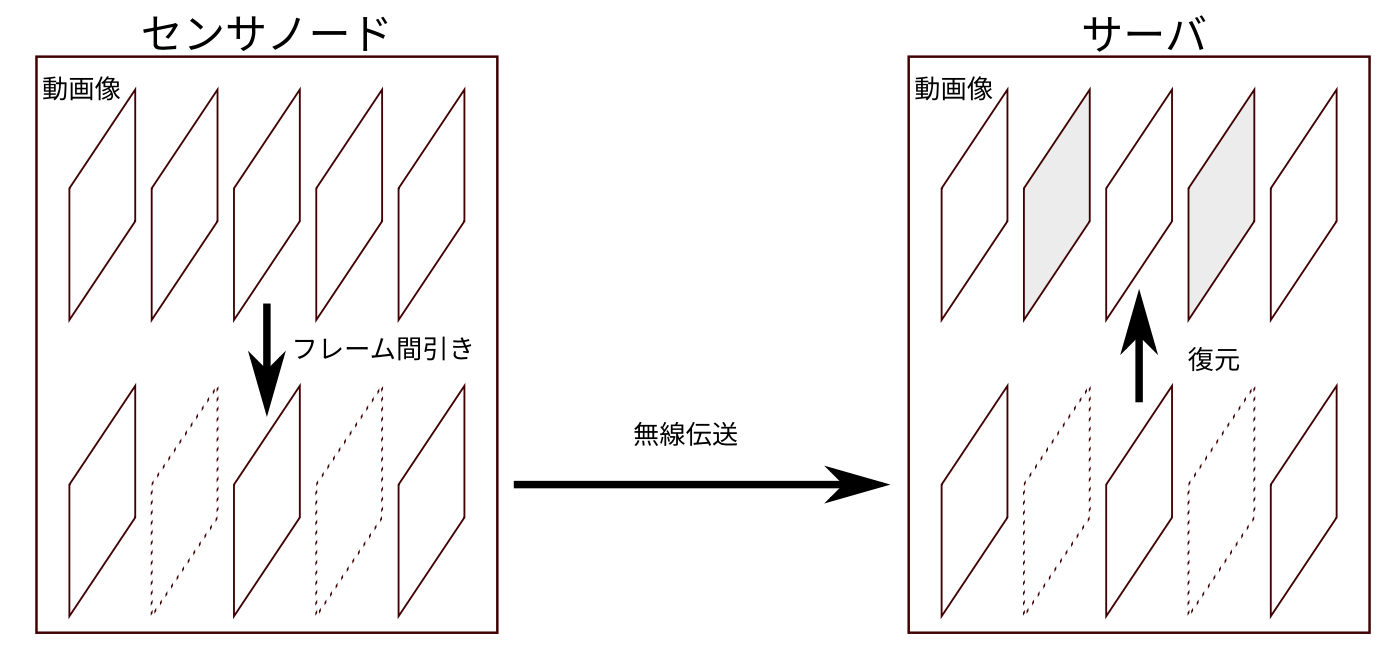
\includegraphics[width=10cm]{./frame_reduction.png}
    \caption{フレーム縮小}
    \label{reduction}
  \end{center}
\end{figure}

\begin{figure}[h]
  \begin{center}
    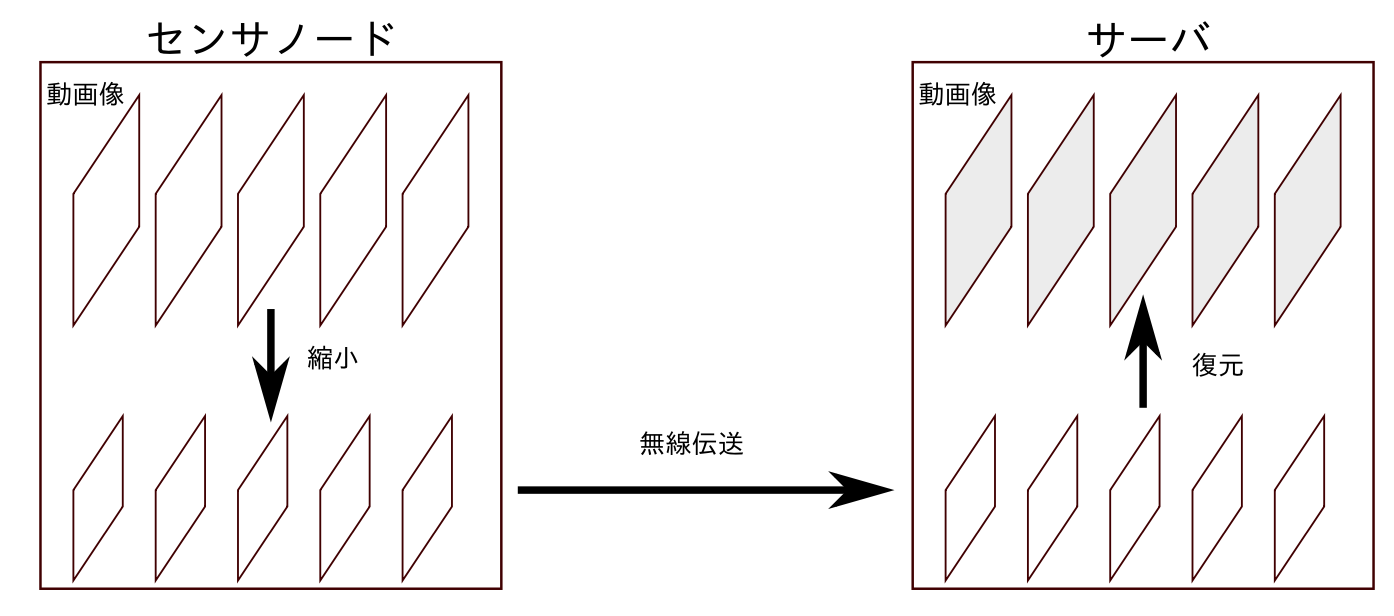
\includegraphics[width=10cm]{./frame_thinning.png}
    \caption{フレーム間引き}
  \end{center}
\end{figure}


動画像のデータ量を削減する最も単純な手法の 1 つとしては,図{}の ように,センサ側で動画像のフレームの解像度を低下させ, サーバ側でそのフレームを復元する方法が考えられる. ここでのサーバ側での復元は,画像の解像度を向上させる超解像と呼ばれる技術の一種になる. 超解像では, 縮小率が大きくなるにつれ, 正確な復元が困難となり, 生成される画像は急激に品質を落とすことになる. そのため, データ量の削減率を大きくしようと縮小率を大きくした場合, 復元された動画像は高周波成分が失われ, 細部を欠いた動画像や, 元の動画像とは異なる動画像を作り出す可能性がある. 超解像とは別の方法として, 図{}のようにセンサ側で動画像のフレームを間引き, サーバ側に渡されたフレームの情報を元に間引かれたフレームを復元するという方法が考えられる. ここでのサーバ側での復元は, 動画像の既存のフレームから新たなフレームを作り出すフレーム補間と呼ばれる技術の一種になる. フレーム補間では, フレームの時間的な間隔が大きくなるにつれ, 動画像内の物体の動きの予測が困難になり, 復元される動画像は動きが不自然になる可能性がある.
どちらの手法も, センサ側では僅かな処理で実現可能であるが, サーバ側では, 動画像の品質を維持するために多大な計算コストが必要になる. これは, 従来の動画像圧縮技術が動画像の送信側に計算コストを置いていたのに対して, 上記の手法が動画像の受信側に計算コストを置いていると考えることができる.

\begin{figure}[h]
  \begin{center}
    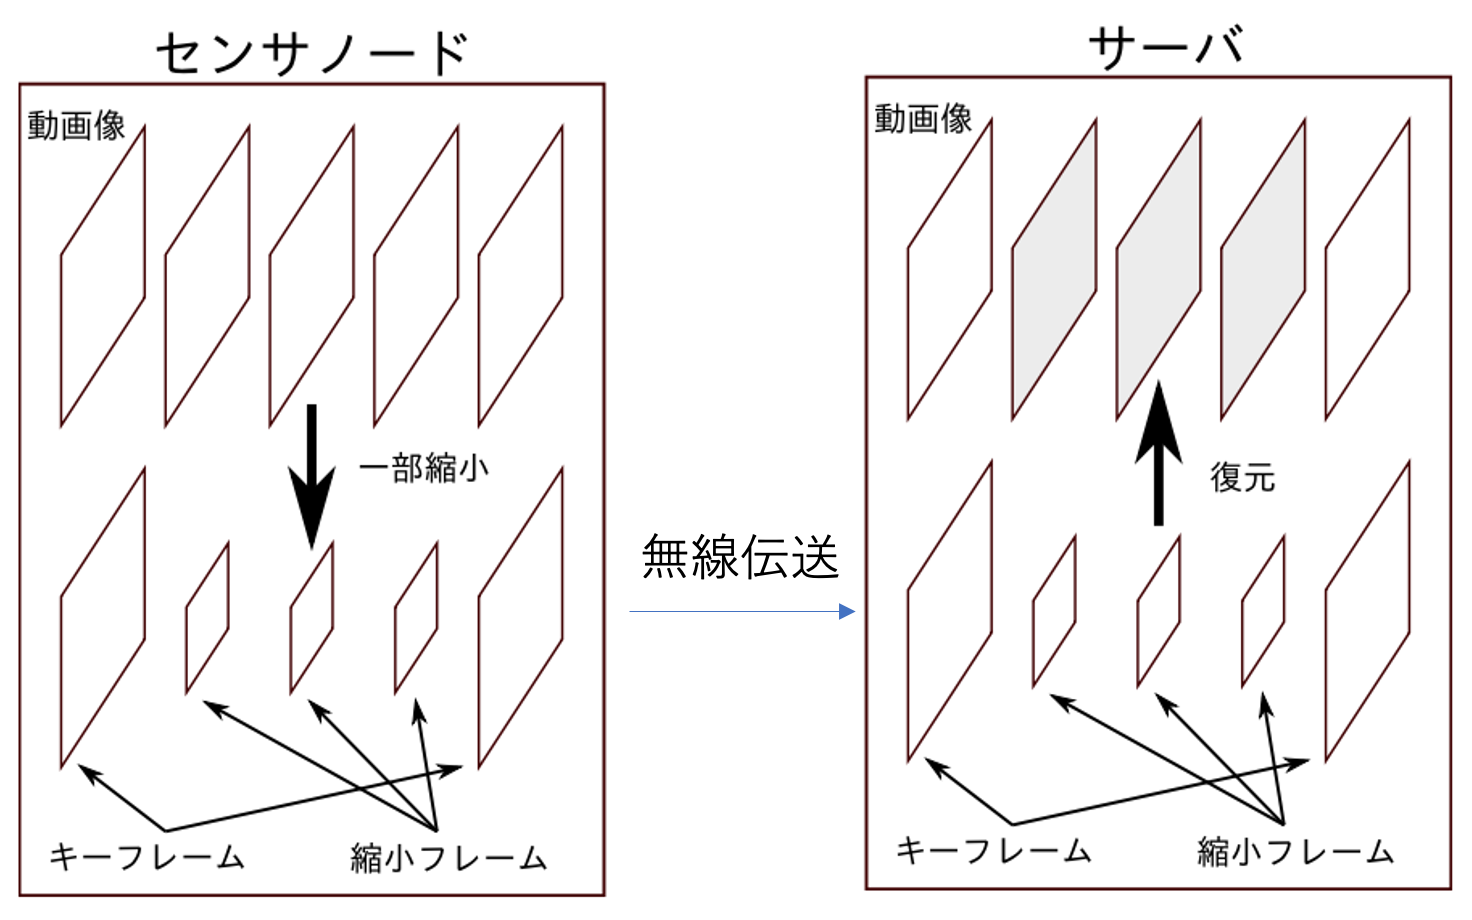
\includegraphics[width=10cm]{./key_thin_frames.png}
    \caption{2種類の解像度のフレームが混在する動画像}
  \end{center}
\end{figure}

近年の論文\cite{Uesaka}で, 複数の解像度のフレームから構成される動画像とその復元手法が提案された. 論文\cite{Uesaka}で提案された動画像は, 図 {}に示すように, キーフレームと呼ばれる高解像度なフレームと縮小フレームと呼ばれる低解像度なフレームの 2 種類の解像度のフレームから構成されており, いくつかの連続する縮小フレームを 2 枚のキーフレームが取り囲んでいる形になっている. センサ側では, 動画像の一部のフレームの解像度を低下させた後に送信を行う. サーバ側の処理は, 受信した縮小フレームとキーフレームが混在する動画像から, キーフレームの情報を用いて, 縮小フレームの復元を行う. この手法では, 全ての解像度を低下させただけの場合や, 一部のフレームを間引き, フレームレートを低下させただけの場合と比べ, より少ないデータ量で同様の品質のフレームを復元することができると示されている.\\
そして近年, 論文\cite{Uesaka}に改良を加えた手法として, 論文\cite{Ukihashi}が提案された. 論文\cite{Ukihashi}では, 前景領域の特定方法としてFgSegNetというニューラルネットワークを用いることで, 補間フレームの背景領域の高精細化が可能と示されている.

本稿の構成は次のとおりである. 2 章では準備として関連研究である超解像とフレーム補間について解説を行った後, 論文\cite{Ukihashi}を既存手法として解説する. また, 画像の評価指標についての解説も行う.  3章では, 提案手法について解説を行う. 4章で提案手法と既存手法の比較を行い, 5 章で 結論を述べる.



\chapter{準備}

この章では,本研究と関係する研究である超解像とフレーム補間について解説した後,論文\cite{Ukihashi}で提案されたフレーム補間手法とその要素技術, また画像の評価指標について説明を行う. 最後に, 既存手法の問題点についてもこの章で解説する.

\section{超解像}
超解像とは,動画や静止画の解像度を上げる画像処理技術である. 
超解像を活用すると, 解像していないぼやけた画像から, より精細な画像を生成することができる. 実際に衛星写真や顕微鏡などに応用され, 光学的なボヤケや解像されていない映像に対してボヤケを改善し, 物体の認識や解析を行うことを目的として使われている.
画像の解像度を向上させる古典的な方法としては, Bilinear 補間や Bicubic 補間といった補間ベースの手法がある. 補間ベースの手法では, 高解像度化によって生み出される画素の値は周辺の画素の値の間の値を取る. 例えば, Bilinear 補間では, 周辺 4 画素の値から線形に補間を行う. Bicubic 補間では, 周辺 16 画素から求められる 3 次関数に従って補間を行う. これらの補間ベースの超解像は高周波成分をもたらさず, ぼやけた画像になる傾向がある.
補間ベース以外の超解像手法としては, 学習型と再構成型がある. 
学習型超解像では, まず解像されているエッジパターンに対して撮像プロセスで生じる劣化をシミュレーションし, 低解像画像を生成する. それを何パターンも学習し, データベース化する. 次に, 入力画像(低解像画像)のエッジを解析し, 学習したデータベースと照らし合わせ, どのパターンと照合するかを解析する. そして, 劣化前のパターンに置き換えることで劣化画像を高精細化する. 学習型超解像のメリットとしては, 単数枚の画像のみで実現可能なことである. デメリットは, 大量のパターンをデータベースとして蓄積する必要性と, パターンに合わない場合に改善が期待できないということである.
再構成型超解像は, 複数枚の低解像の画像から, 高解像度の画像を推定する技術である.
再構成型超解像のメリットとしては, 結果画像の破綻が少なく解像度の向上を行いやすいことが挙げられる.デメリットとしては, 複数枚の画像を扱うため, 画像間での画素毎の位置合わせを行う必要性や, 複数の画像データにアクセスするため, 学習型に比べより多くの演算処理性能とメモリ容量を必要とすることが挙げられる.
近年では, 深層学習の登場により, ニューラルネットワークを用いた超解像手法が従来の超解像手法より優れているとして, 非常に注目を集めている. (ココいらんかも)


\section{フレーム補間}
フレーム補間とは, 時間的に隣接するフレームの間に, 新たにフレームを作り出す技術である. 本研究は, 高解像度フレームの情報を使い, 縮小フレームに対応するフレームを生成するという意味で, フレーム補間技術の一つだと考えることができる. 本節では, 基本的なフレーム補間技術について解説する. フレーム補間の基本的な考え方は, 既存のフレームから新たに作り出すフレームへの画素の動きを推測し, 既存フレームの画素を移動させることで新たなフレームを生成するという処理である. この動きの推測は optical flow と呼ばれる.  optical flow には様々な手法が存在し, フレーム補間以外にも動画の圧縮など様々な分野で用いられる.
近年では, 超解像と同様にフレーム補間の分野でも深層学習を用いた手法が注目を集めている.


\section{2 種類の解像度のフレームを混在させた動画像の特徴点補間による復元}
この節では,2 種類の解像度のフレームを混在させた動画像の特徴点補間による復元\cite{Ukihashi}について解説する. なお, 論文\cite{Ukihashi}の2つ目の提案である深層学習を用いた補間手法は, 本稿では取り扱わないため, 解説は割愛する.  既存手法のフレーム補間は,特徴点マッチングとホモグラフィ変換を用いることで達成される. 補間処理の概要を図[] に示す. 

\begin{figure}[h]
  \begin{center}
    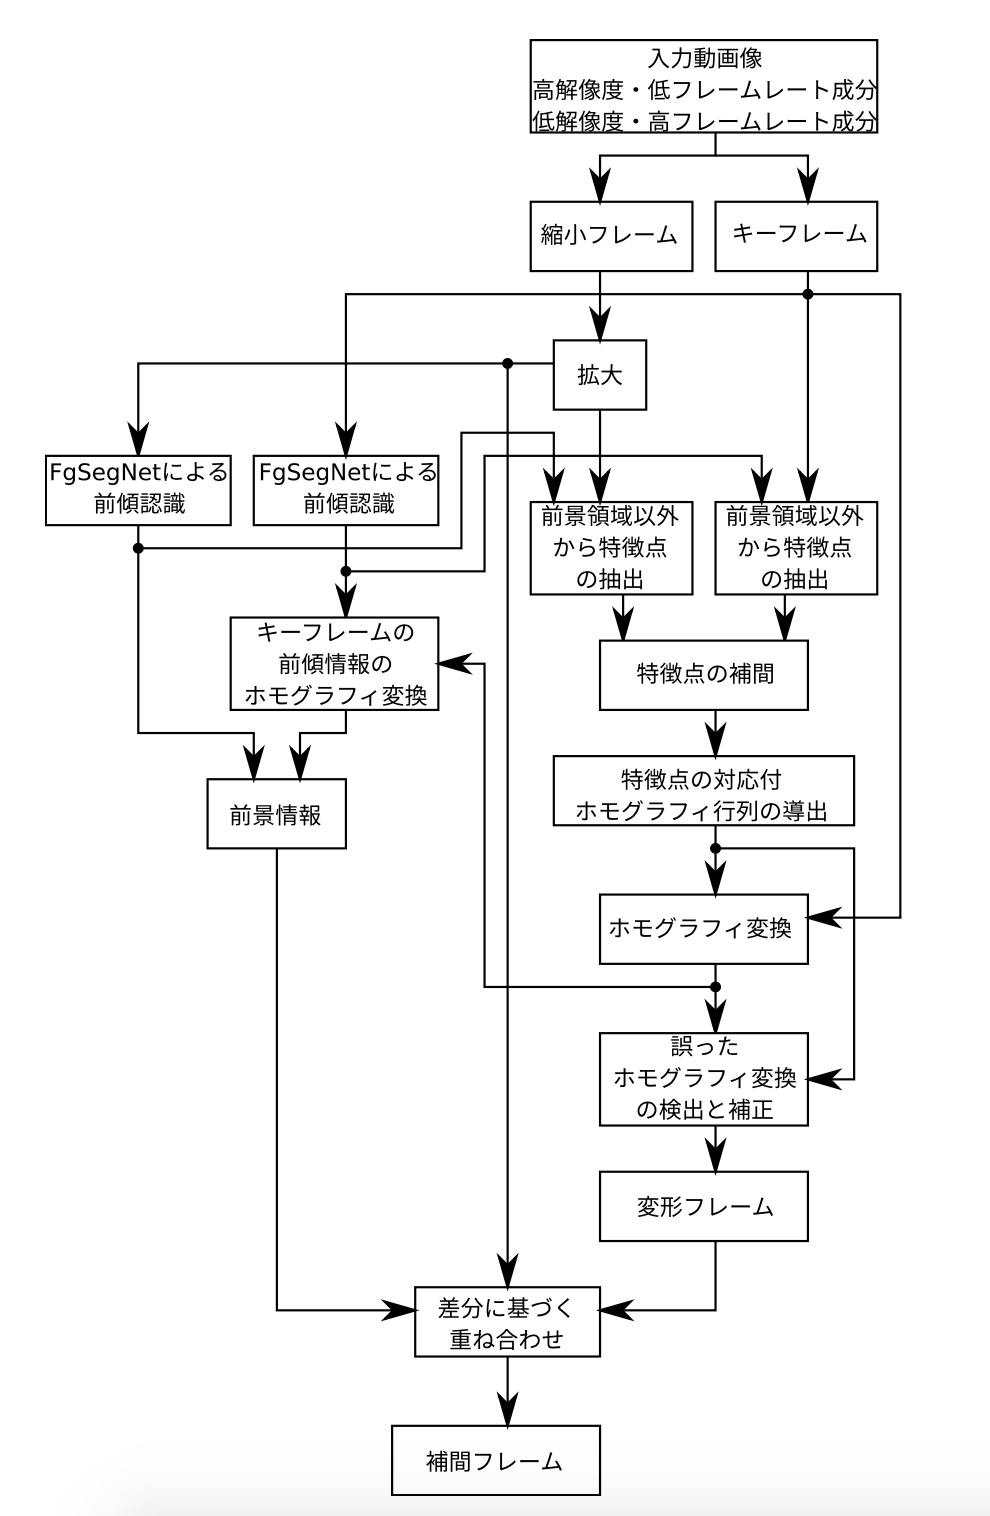
\includegraphics[width=8cm]{./kizonshuhou_zentaizou.png}
    \caption{2 種類の解像度のフレームを混在させた動画像の特徴点補間による復元}
  \end{center}
\end{figure}

既存手法では, まず,縮小フレームを bilinear 補間や bicubic 補間といった単純な超解像手法で解像度を復元した拡大フレームを生成する. これらの拡大手法は高周波数成分をもたらさず,拡大フレームは細部を欠いた ぼやけたフレームとなる. より高い品質のフレームを得るためには,キーフレームに存在する情報を用いてより高精細なフレームにする必要がある. 
キーフレームを拡大フレームの時刻のものに変形するために,まず,キーフレームと拡大フレームから特徴点と呼ばれる画像中に存在する特徴的な点を抽出する. 特徴点を抽出するアルゴリズムは様々なものが存在するが,基本的に画像内のコーナーが特徴点の候補となる. 特徴点の抽出後,キーフレーム内の特徴点と拡大フレーム内の特徴点で対応関係を見つける. この作業を特徴点マッチングという. 
特徴点マッチングは,特徴点の周辺の画素を目印として行われる. この対応関係は,特徴点の optical flow を表していると考えることができる. 一般的なフレーム補間に用いられる optical flow との違いとして,一般的なフレーム補間で用いる optical flow は全ての画素のフローであるのに対して, 特徴点マッチングは, フレーム内の特徴点のみのフローとなる. また, 一般的なフレーム補間は, 動きが線形に補間できるということを前提とし, optical flow を線形にスケーリングさせ,新たなフレームへの optical flow を作り出していた. 
しかし既存手法では, 2 種類の解像度のフレームが混在する動画像を用いているため,縮小フレームへの直接的な optical flow を求めるだけでよく,動きが線形に補間できるという前提の必要性がなくなった点が異なる.

上述の処理によってキーフレームから拡大フレームへの特徴点のフローは得られるが,特徴点以外の画素のフローが存在しない. そこで,特徴点マッチングの情報からホモグラフィ行列の推定を行う. ホモグラフィとは 2 平面に関する投影を表す. キーフレームに存在する画像を拡大フレーム上の適切な位置に投影することで,拡大フレームのぼやけている領域をキーフレームの精細な情報と置き換えることができる. ホモグラフィ行列の推定は,特徴点の疎な optical flow から, 画像上の画素全てに対する密な optical flow の推定と考えることができる. この手法による高精細化は,2 つのフレームの関係が 2 平面の投影で表現できるということを前提としている. つまり, フレームに写っている個々の物体が別々の速度を持っている場合や,ある物体が一方のフレームにしか写っていない場合 等は成り立たない. このように上記の前提が成り立たない場合,ホモグラフィ行列の推定ができないため, その領域は拡大フレームの高精細化には利用できない. そこで既存手法では,FgSegNet[]と呼ばれるニューラルネットワークを用いて, 高精細化に利用できない領域を検出している. FgSegNet とは動画像中の動いている物体の領域を検出するニューラルネットワークである. このような動く物体のことを前景と呼ぶ. つまり, 前景領域を特定することで, それ以外の領域の高精細化を可能としている.

高精細化に利用できない領域をさらに正確に検出するために, 既存手法では, 以下の3つの処理を行う. 
1つ目は, 前景領域からの特徴点の除去である. ホモグラフィ行列は特徴点マッチングの情報から推定される. ここで,ホモグラフィ行列の推定の際に, 前景領域の特徴点と背景領域の特徴点が混在した情報源を利用すると, 推定されるホモグラフィ行列は前景の動きと背景の動きが混ざった動きを表現したものになる. また,背景の特徴点に重なるように前景が動いた場合,利用できる特徴点の数が減り,ホモグラフィ変換の低精度化につながる. そこで既存手法では, FgSegNetによって検出した前景領域の情報を参照し,  特徴点マッチングの情報から, 前景領域の特徴点を除去する. こうすることで, 背景の動きのみを表すホモグラフィ行列を推定できる.
2つ目は, 特徴点の補間である. 上述のように, 利用できる特徴点の数が減ると, ホモグラフィ変換の低精度化につながる. そこで,他のフレームからホモグラフィ変換を用いて特徴点を射影することによって,利用できる特徴点を増やし,より高精度なホモグラフィ推定を行う. 
3つ目は, 誤った推定がされたホモグラフィ行列の検出である. 精度の低いホモグラフィ行列を用いると, 補間フレームの品質を大きく損なう. そこで, ホモグラフィ行列の精度を確かめ, 精度が低い場合はそのホモグラフィ行列を使用しないという判断をする. 精度の低いホモグラフィ行列を使用しない場合,正常なホモグラフィ行列を用いた場合と比べると, 補間フレームの品質を大きく損なうが,最低でも拡大フレームの品質は保証できることになる.

最後に, これまで取得した各フレームの差分に基づく重ね合わせを行う. 
重ね合わせは, 式[]に示すモデルを使用している. 

\begin{equation}
 I(x,y) = (1 - \alpha)T_0(x,y)+\alpha T_1(x,y)\\ 
\end{equation}
$$ \alpha = \frac{d0}{d0+d1} \\ $$
$$ d_0 = |E(x,y) - T_0(,x,y)|, d_1 = |E(x,y) - T_1(,x,y)| $$

式[] の E(x, y) は拡大フレームの画素を表し,拡大フレームの画素 とキーフレームの画素の差分が小さい方がより強く補間フレームに反映されるということを意味している. 式[]を用いることで,画素単位での重ね合わせの比率を決定することができ,より柔軟な重ね合わせを期待できる.



\section{特徴点マッチング}
特徴点マッチングとは, 画像上の特徴点を抽出し, 2枚の画像間の共通する特徴点を対応づける技術である. 主な構成は特徴点検出, 特徴量記述, マッチングの3段階からなる. 特徴点検出では, 画像中から角や線の交わり, エッジなどの他と区別できるような固有の点の座標を検出する. 特徴量記述では, 検出した特徴点の固有性をベクトルやバイナリコードで表現した値の特徴量として算出する. マッチングでは, 対応付ける画像同士の特徴量を比較する. 特徴量の距離が近いものを類似度が高いと判断し, 特徴点を対応付ける. 図[]の丸印は, その画像上の特徴点を表している. 図[]は, 図[]をグレースケール変換した後, 特徴点抽出,特徴量記述を行い, 図[1]の特徴点とマッチングをしたものを表している. 
\begin{figure}[h]
  \begin{center}
    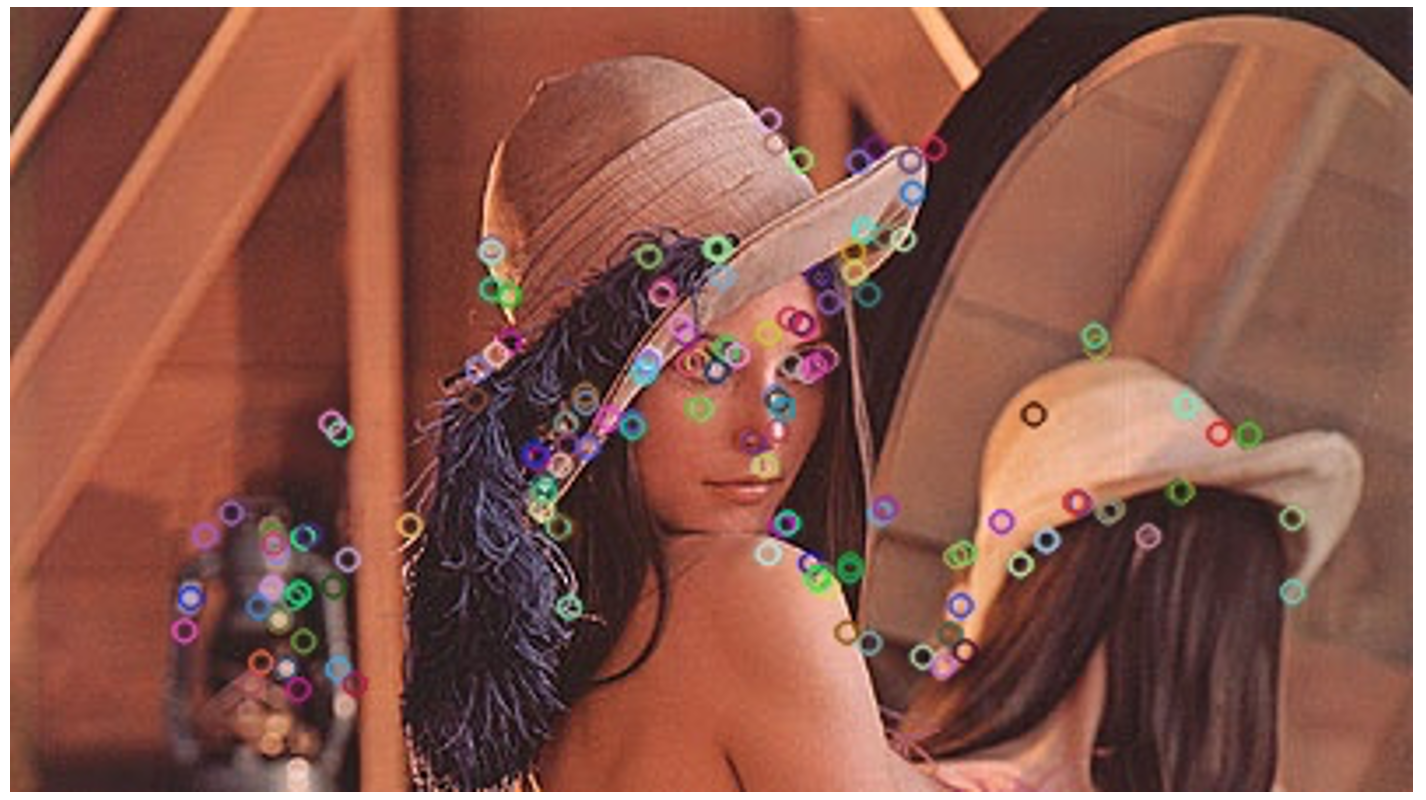
\includegraphics[width=10cm]{./lena_featurepoints.png}
    \caption{特徴点の抽出}
  \end{center}
\end{figure}

\begin{figure}[h]
  \begin{center}
    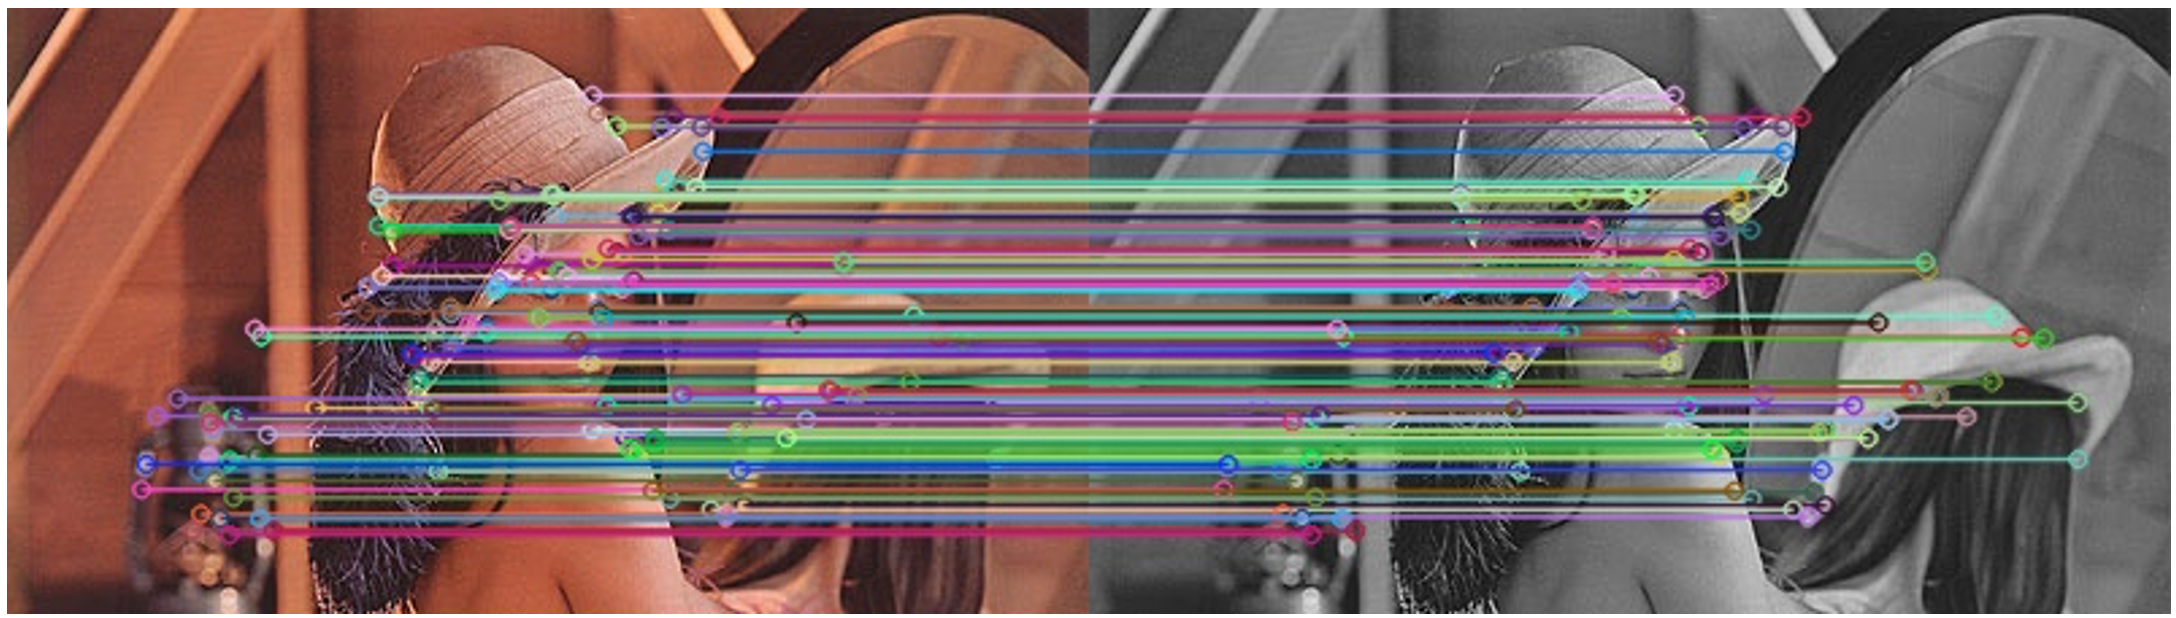
\includegraphics[width=10cm]{./features_match.png}
    \caption{特徴点マッチング}
  \end{center}
\end{figure}



\section{ホモグラフィ変換}
\(
2.3節で述べたようにホモグラフィ行列を推定した後, 実際にある平面を別の平面に投影することを, ホモグラフィ変換という. 図[]のように, ホモグラフィ変換を行った画像は, 任意の形に変形することができる. この変換はまず,3 次元空間 (x,y,z) 上の平面 (x,y,1) 上に存在する投影元の平面に対して線形変換をかける. この線形変換された投影元の平面を, 原点 (0,0,0) を焦点として平面 (x,y,1) に投影する. ここで平面 (x,y,1) に投影された画像が, ホモグラフィ変換後の画像となる. 線形変換前の画像上の点 p に線形変換を行った点を 点p′,点 p′ を平面 (x,y,1) に投影した点を点q とする. この時, 原点を焦点とした平面 (x,y,1) への投影は,図[]より,原点O, 点q, 点(0, 0, 1) から できる三角形と原点O, 点p′, 点(0, 0, z′) からできる三角形が相似である. これより,原点を焦点とした平面 (x,y,1) への投影は, 投影元の平面の z 座標で割ることで得られることがわかる. まとめると, ホモグラフィ変換は以下の式で定義できる. 
\)
\[
	p=\left(
		\begin{array}{c}
			x \\
			y \\
			1 \\
		\end{array}
	\right),
	p'=\left(
		\begin{array}{c}
			x'\\
			y'\\
			z' \\
		\end{array}
	\right),
	p'=\left(
		\begin{array}{c}
			X\\
			Y\\
			1\\
		\end{array}
	\right)
\]
\[
	H = \left(
		\begin{array}{ccc}
			h_{11} & h_{12} & h_{13}\\
			h_{21} & h_{22} & h_{23}\\
			h_{31} & h_{32} & h_{33} 
		\end{array}
	\right)
\]
$$ p' = Hp \\$$
$$ q = \frac{1}{z'}p' \\$$
$$X = \frac{h_{11}x + h_{12}y + h_{13}}{h_{31}x + h_{32}y + h_{33}}, Y = \frac{h_{21}x + h_{22}y + h_{23}}{h_{31}x + h_{32}y + h_{33}} \\$$


しかし,X, Yを見ると分子と分母には定数がなく, 冗長である. そこで,式[]に示すように,X, Yを $h_33$ で割ることでより簡潔に表現でき,ホモグラフィ行列の自由度は 8 となる.
$$X = \frac{h'_{11}x + h'_{12}y + h'_{13}}{h'_{31}x + h'_{32}y + 1}, Y = \frac{h'_{21}x + h'_{22}y + h'_{23}}{h'_{31}x + h'_{32}y + 1} \\$$
最終的に推定されるホモグラフィ行列を式[]に示す.この 8 つの変数を推定することにより,ホモグラフィ推定が達成される.
\[
	H = \left(
		\begin{array}{ccc}
			h_{11} & h_{12} & h_{13}\\
			h_{21} & h_{22} & h_{23}\\
			h_{31} & h_{32} & 1 
		\end{array}
	\right)
\]
ホモグラフィ行列は自由度 8 の行列であるため,この行列の推定には 2 枚 の画像の対応する点のペアが 4 組が必要となる.この 4 組の点のペアか ら direct linear transformation (DLT) アルゴリズムを用いて,ホモグラフィ行列を推定する.しかし,よりロバストなホモグラフィ行列の推定を行うために 4 組以上の点のペアと RANSAC 法を用いてホモグラフィ行列を推定する方法なども用いられる. 既存手法では,得られた複数の特徴点のペアから RANSAC 法を用いてホモグラフィ推定を行っており, 本稿の提案手法でも同じ手法を用いている.
\begin{figure}[h]
  \begin{center}
    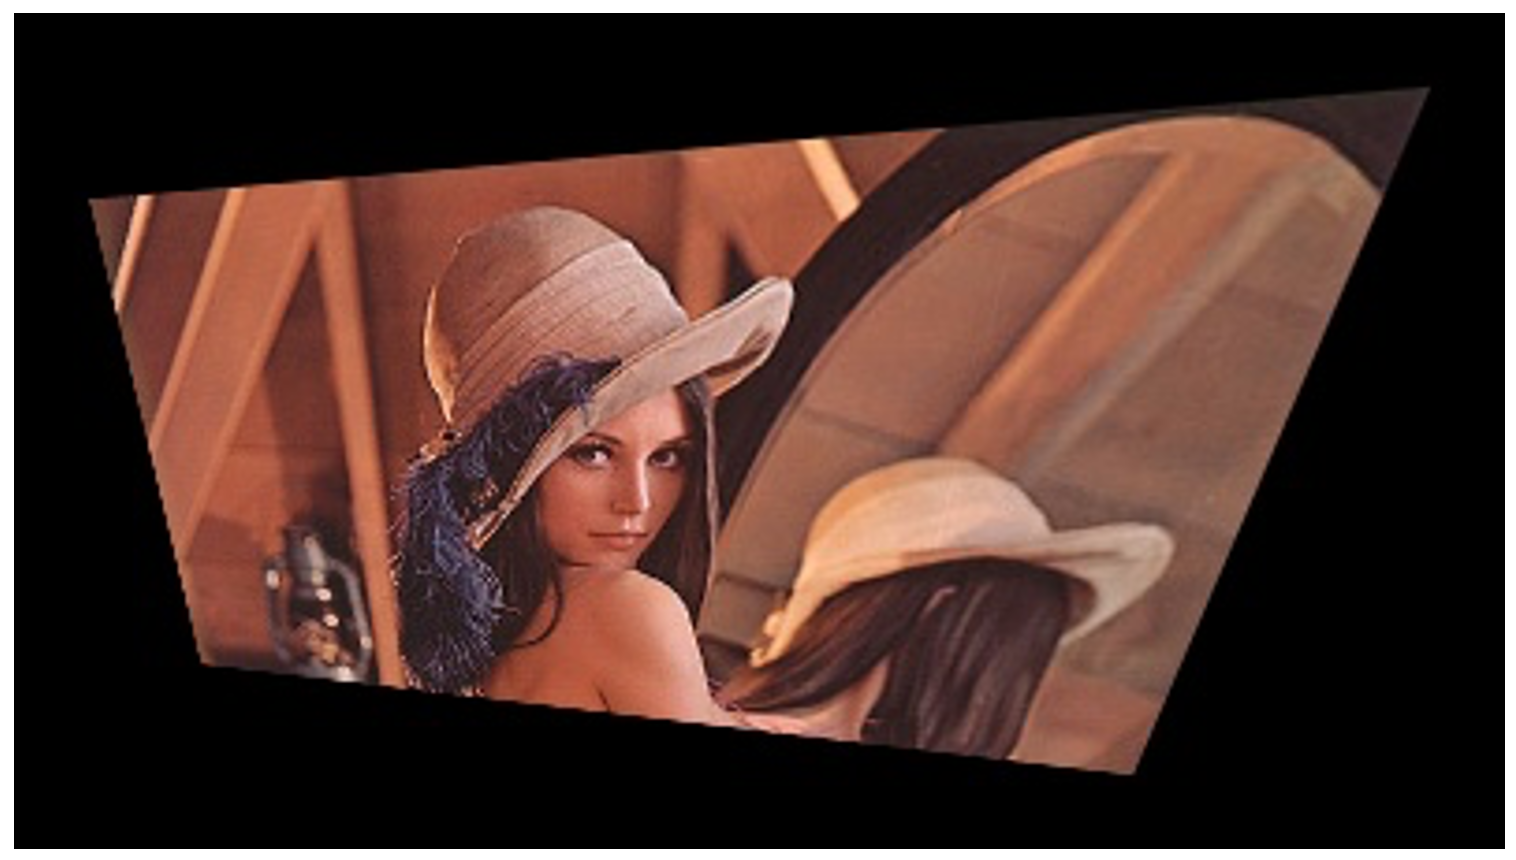
\includegraphics[width=10cm]{./homography_transformation.png}
    \caption{ホモグラフィ変換}
  \end{center}
\end{figure}



\section{画像の評価指標}
画像を評価する方法は, 主に客観評価と主観評価に分けられる. 客観評価は, 原画像と処理画像による数値的な比較による評価である. 主観評価は, 人間の視覚による感覚的な評価である. 
人間が歪んだ画像に対する評価を自動的に予測するアルゴリズムとして, IQAモデルというものがある. IQAモデルは, 比較のための参照画像を用いるかどうかで2つに分けらる. 参照画像を用いる方を, FR-IQAまたは客観的指標と呼び, 参照画像を用いない方を, NR-IQAまたは主観的指標と呼ぶ. 本研究では, 主観的指標を新たな評価指標として加えるため, その一つであるNIQE\cite{6353522}というモデルを利用する. 本節では, NR-IQAおよびNIQEについての解説を行う. 

\section{NR-IQA}
NR-IQAとは, 画像に対する人間の主観的な評価を予測するものである. 測定の際は一般に, FR-IQAが原画像と処理画像の2つを用いるのに対し, NR-IQAは, 処理画像のみを用いる. 一般的なNR-IQAモデルは, 人間が評価した処理画像とその評価値のデータベースに基づき, 人間による画質の評価値の予測方法を学習する. このようなNR-IQAモデルは, 学習済みの歪みタイプによる品質の低下しか評価できない. このように, NR-IQAモデルは, どのようなデータを学習に用いるかで分類することができる. 
NR-IQAモデルを大別すると, OAとOUに分けられる. OUはさらに, DAとDUに分けられる.
人間が評価した処理画像とその評価値のデータベースで学習されている場合, 'OA' (opinion - aware)に分類される. そのようなデータベースを学習に用いていない場合は, 'OU' (opinion - unaware) に分類される. ただし, OUに属するモデルは, 予測される歪みに関する知識が予め必要となる. 同様に, OU型のモデルから派生したIQAモデルは, 処理画像をIQAモデルの作成または学習に利用できるかどうかで分類される. 例えば, 学習用の画像が不十分な環境では, 歪みに関する情報を取得するのが難しい. このとき, 特定の歪みタイプに特化した学習をし, その歪みタイプを定式化するIQAモデルは, 'DA' (distortion - aware)に分類される. 一方, 特定の歪みタイプに特化せず, 未加工の自然画像またはその画像モデルのみで学習するIQAモデルは, 'DU' (distortion - unaware)に分類される. 


\section{NIQE}
一般的なNR-IQAモデルでは, 人間が評価した歪み画像とその評価値のデータベースや, 特定の歪みタイプを学習する. しかし, NIQEは, このようなデータベースも特定の歪みタイプの事前訓練も必要としない, いわゆるOU-DU型のNR-IQAモデルである. NIQEでは, このような人間の評価や画像の特定の歪みタイプではなく, NSS(Natural Scene Statics)に着目している.
NSSというのは,  自然画像に見られる統計的な規則性のことであり, これをベースにすることで, より画像の'品質'に着目したモデルになっている. NSSに基づき構築したモデルを多変量ガウスモデルに適合させ, テスト画像でも同様に, NSSベースのモデルを作成し, 多変量ガウスモデルに適合させる. 自然画像とテスト画像のそれぞれの多変量ガウス適合間の距離が, テスト画像の評価値とされる. 
以下, NIQEの主な5つの構成要素を説明する. 

1つ目は, 空間ドメインNSS特徴の抽出である. 空間ドメインNSS特徴とは, NIQEのモデル構築のベースとなる特徴量であり, 画像の視覚的な品質に関わる. 古典的な導出方法は, 式2.2のように, 最初に局所平均除去と分割正規化を行う. 
\begin{equation}
 I(i,j) = \frac{I(i,j) - \mu(i,j)}{\sigma(i,j) + 1}\\ 
\end{equation}
 \begin{equation}
 \mu(i,j) = \sum_{k=-K}^K \sum_{l=-L}^L \omega_{k,l} I(i+k, j+l)\\ 
\end{equation}
\begin{equation}
 \sigma(i,j) = \sqrt{\sum_{k=-K}^K \sum_{l=-L}^L \omega_{k,l} [I(i+k, j+l)-\mu(i,j)]^2}\\ 
\end{equation}
i,j は空間インデックスを表しており, 式,式はそれぞれ局所平均とコントラストを推定している. $$\omega$$は円対称ガウス関数を表しており, これで重み付けをする. 歪みが全くない自然画像から求めた空間ドメインNSS特徴はガウス分布に従うが, 歪みを含む画像の場合は, その歪みの程度に応じてガウス分布からのずれが生じる. つまり, ガウス分布との類似度が,  画像の品質を評価する際の重要な指標となる.

2つ目は, パッチ選択である. 式を計算した後, 画像はPxPパッチに分割され, 各パッチの分散を基準に選択していく. 視覚的品質は被写体のコーナーの部分の鮮明さに基づいていると言われており, 分散は鮮明さと言い換えられるためである. 被写体のコーナーの例を図[]で示すと, 赤枠で囲まれた領域がそれにあたる. 図[]より, 水面と山の境目・人と水面の境目・空と山の境目といった部分が選択されていることがわかる. この部分が鮮明であれば, 水面が多少ぼやけていても, 人間は綺麗な画像だと評価される. 逆に水面がとても鮮明な画像でも, コーナーの部分がぼやけていれば人間にとって綺麗な画像とは評価されないということとなる. 

\begin{figure}[h]
  \begin{center}
    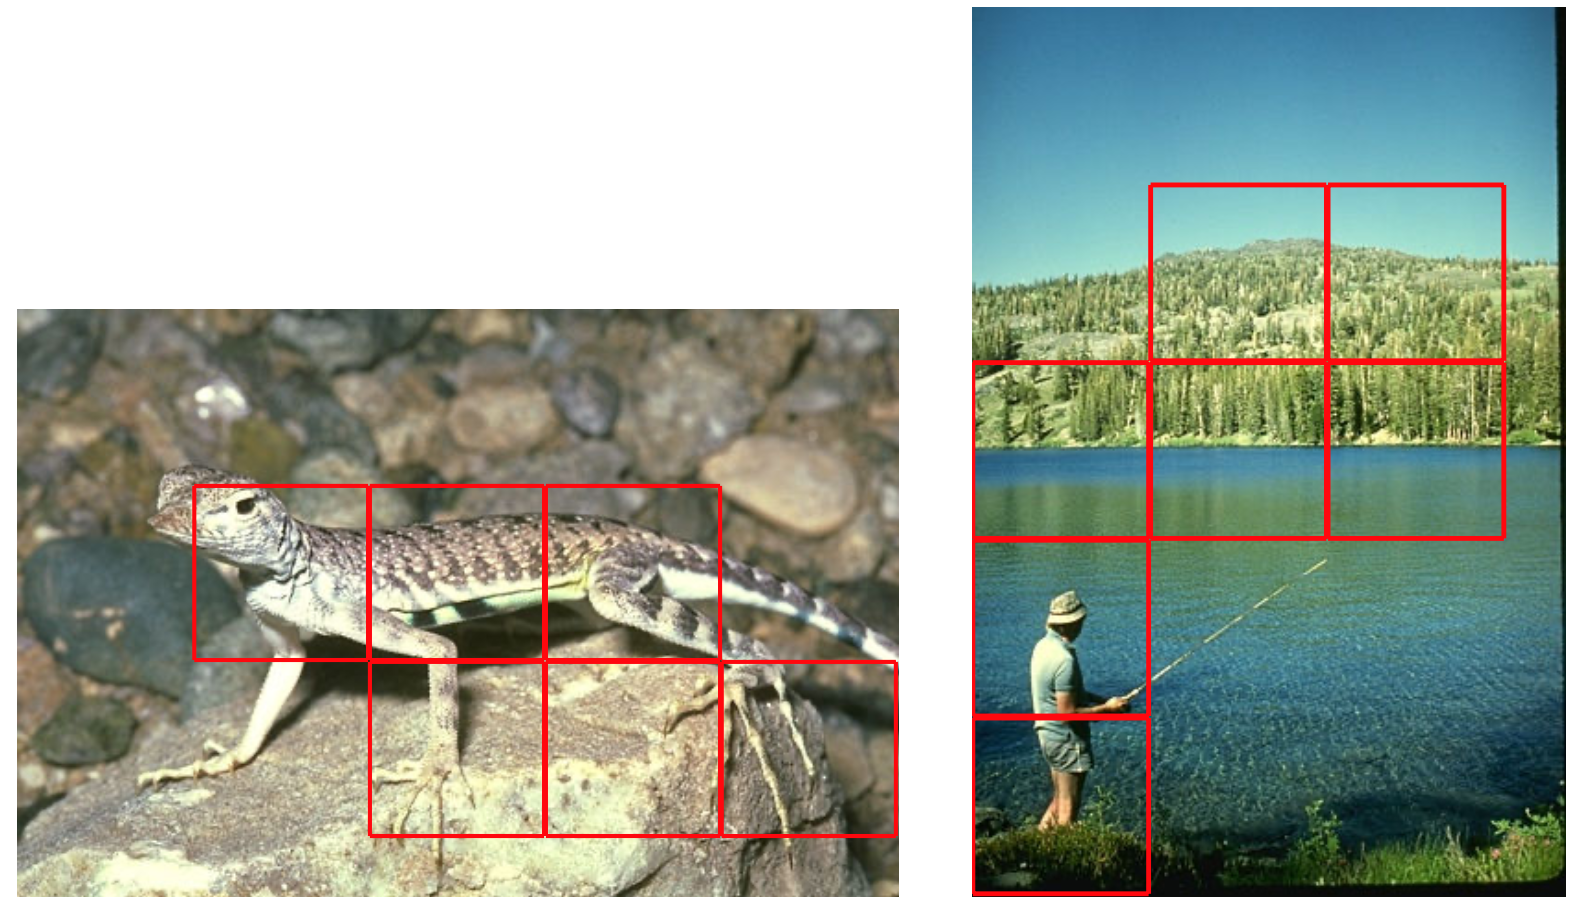
\includegraphics[width=10cm]{./NIQE.png}
    \caption{被写体のコーナー}
  \end{center}
\end{figure}

各パッチの分散は式[]で求められる. 各パッチの分散値を求めた後, 値が大きく, 歪みの発生確率が低いパッチを優先的に選択していく. このパッチのサブセットを用いて, 自然画像パッチの統計モデルを構築する.
\begin{equation}
 \delta(b) = {\sum \sum}_{(i,j)\in patchb } \sigma(i,j)\\ 
\end{equation}

3つ目は, パッチの特徴づけである. 自然画像パッチのサブセットが与えられると, 各パッチから計算された'品質を意識した'NSSによって特徴づけが行われる. NSSベースの画質に関する先行研究により, 一般化ガウス分布が式の係数の挙動を推定できることがわかっている. 平均が0の一般化ガウス分布(GGD)を式に示す.
\begin{equation}
 f(x;\alpha, \beta) = \frac{\alpha}{2\beta\Gamma(1/\alpha)}\exp{(-(\frac{|x|}{\beta})^\alpha)}\\ 
\end{equation}

式で求めた値の符号は, 自然画像では規則性が見られるが, 歪み画像の場合は, 歪みの度合いに従って規則性が乱れていく. この自然像と歪み画像との偏差は, 隣接係数の積の分布を分析することで推定できる. この隣接係数の積は, 非対称一般化ガウス分布(AGGD)に従うようにモデル化されている. また, ここで分散の平均も求める. AGGD, 分散の平均値を式,式に示す.

\begin{eqnarray}
f(x;\gamma,\beta_l,\beta_r)=
	\begin{cases}
			\frac{\gamma}{(\beta_l + \beta_r)\Gamma(1/\gamma)}\exp{(-(\frac{-x}{\beta_l}))^\gamma} \forall x \le 0&\\
			\frac{\gamma}{(\beta_l + \beta_r)\Gamma(1/\gamma)}\exp{(-(\frac{x}{\beta_l}))^\gamma} \forall x \ge 0&
	\end{cases}
\end{eqnarray}

\begin{equation}
 \eta = (\beta_r - \beta_l)\frac{\Gamma(2/\gamma)}{\Gamma(1/\gamma)}\\ 
\end{equation}

4方向に沿って式~式を計算することで, 16個のパラメータが得られ, 式と式を含めると全体で18個のパラメータが得られる. これら全ての特徴は, マルチスケールの挙動を推定するために, 2つのスケールで計算され, 最終的に36個のパラメータが生成される. 


4つ目は, 多変量ガウスモデルへの適合である. 上述で求めた36個のパラメータを多変量ガウスモデル(MVG)にフィッティングさせ, NSS特徴の単純モデルを取得する. 

\begin{equation}
 f_X(x_1, ..., x_k) = \frac{1}{(2\pi)^{k/2}|\sum|^{1/2}}\exp{(-\frac{1}{2}(x-\nu)^T\sum^{-1}(x-\nu))}\\ 
\end{equation}

ここで$$(x_1, ... , x_k)$$は, 式~式で求めたNSS特徴であり, $$\nu, \sum$$はそれぞれMVGモデルの平均と共分散行列を表している.


最後に, 多変量ガウスモデルに適合させたモデル間の距離を求める. 
上述までの流れをまとめると, 自然画像をPxP個のパッチに分割し, 選択されたパッチから36個のパラメータを求め, それらをMVGモデルに適合させることで, 単純なNSS特徴モデルを作成する.この作業をテスト画像でも同様に行い, 特徴モデルを作成する. 
テスト画像を評価する時は, 自然画像から取得したNSS特徴モデルとテスト画像から取得した特徴モデル間の距離を求める. 距離を求めるには, 式を用いる.
$$\nu_1, \nu_2および\sum_1, \sum_2$$は, 自然画像のNSS特徴モデルと歪み画像の特徴モデルの平均ベクトルと共分散行列を表す. 

\begin{equation}
 D(\nu_1,\nu_2,\sum_1,\sum_2) = \sqrt{((\nu_1-\nu_2)^T(\frac{\sum_1+\sum_2}{2})^{-1}(\nu_1-\nu_2))}\\ 
\end{equation}




\section{既存手法の問題点}
本節では,論文\cite{Ukihashi}の問題点について説明する.

\subsection{客観的指標のみによる評価}
既存手法では, 補間フレームの背景領域の高精細化を目的としていた. しかし, 生成された補間フレームの評価は, PSNR,つまり客観的指標のみに基づいたものであり, 主観的な評価がなされていない.  実際に生成された補間フレームを見ると, 図[]のように, 前景領域と背景領域の境目の不自然さや, 前景領域のぼやけが目立つ. また, オリジナル画像と補間フレームをPSNRとNIQEの値で比較してみると, 確かにPSNRにおいては既存手法が優れているが, NIQEにおいては劣っていることがわかる. 
\begin{figure}[h]
  \begin{center}
    \includegraphics[width=10cm]{./ukihashi_method.bmp}
    \caption{既存手法による補間フレーム}
  \end{center}
\end{figure}

\begin{figure}[h]
  \begin{center}
    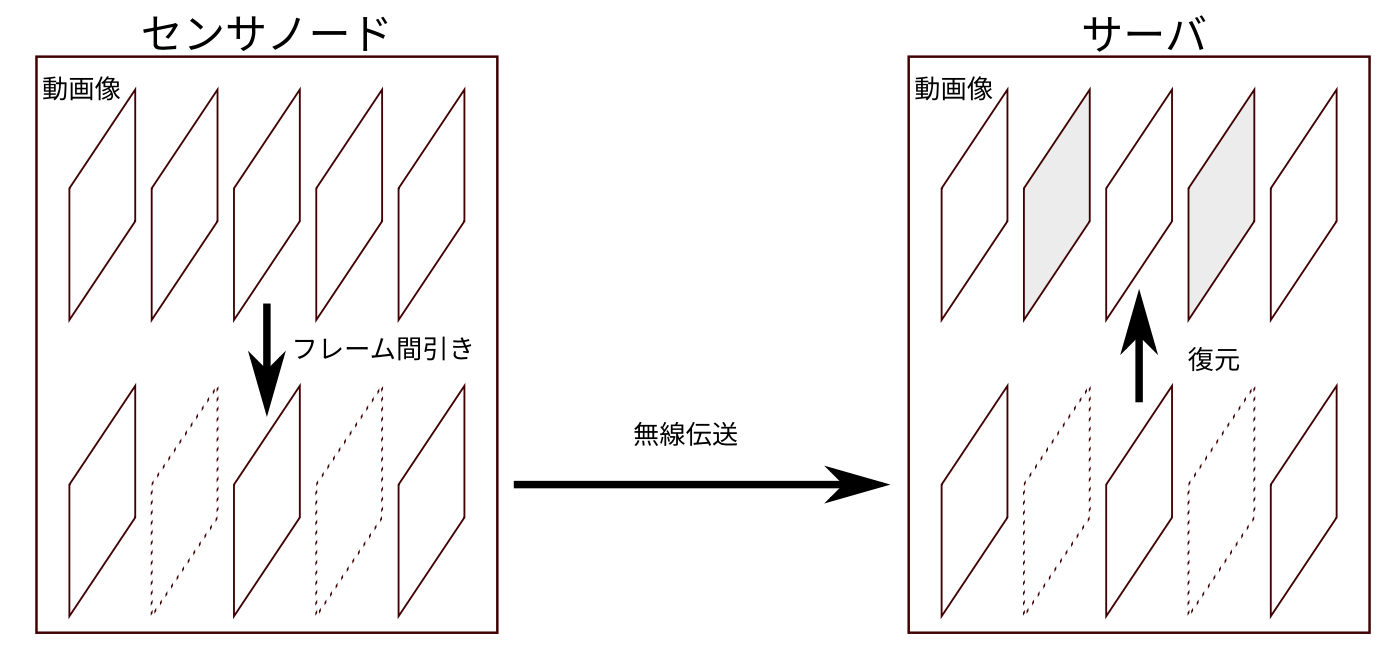
\includegraphics[width=10cm]{./frame_reduction.png}
    \caption{既存手法のPSNRとNIQE}
  \end{center}
\end{figure}


\subsection{前景領域の特徴点の削除}
既存手法の別の問題点として, 前景領域の特徴点を削除していたことが挙げられる. 
ホモグラフィ行列は, キーフレームと拡大フレームの画像間から取得した特徴点マッチングの情報を用いて導出される. 図[]のように, 特徴点は, その座標がベクトルに格納されている. 2.3節で述べたように, 特徴点マッチングを行った直後では, 前景領域の特徴点と背景領域の特徴点が混在した状態になっている. この状態のベクトルからホモグラフィ行列を導出すると, 前景の動きと背景の動きが混ざったものを表現することになり, ホモグラフィ変換の低精度化に繋がる. 
そこで既存手法では, ホモグラフィ行列を求める前に, 前景領域の特徴点を削除している. 背景領域の特徴点のみで構成されるベクトルからホモグラフィ行列を求めることで, 背景の精細化を可能としている. しかし, 背景領域の特徴点のみから求めたホモグラフィ行列では, 図[]のように, 前景の位置がほとんど移動せず, 拡大フレームの前景領域の高精細化はできない. そのため, 図[]のように, 補間フレームの前景領域は, 拡大フレームの情報をそのまま用いており, 前景のみがぼやけたフレームになっている. 
以上の理由から, 既存手法は前景領域の主観的品質において改善の余地がある. 


\begin{figure}[h]
  \begin{center}
    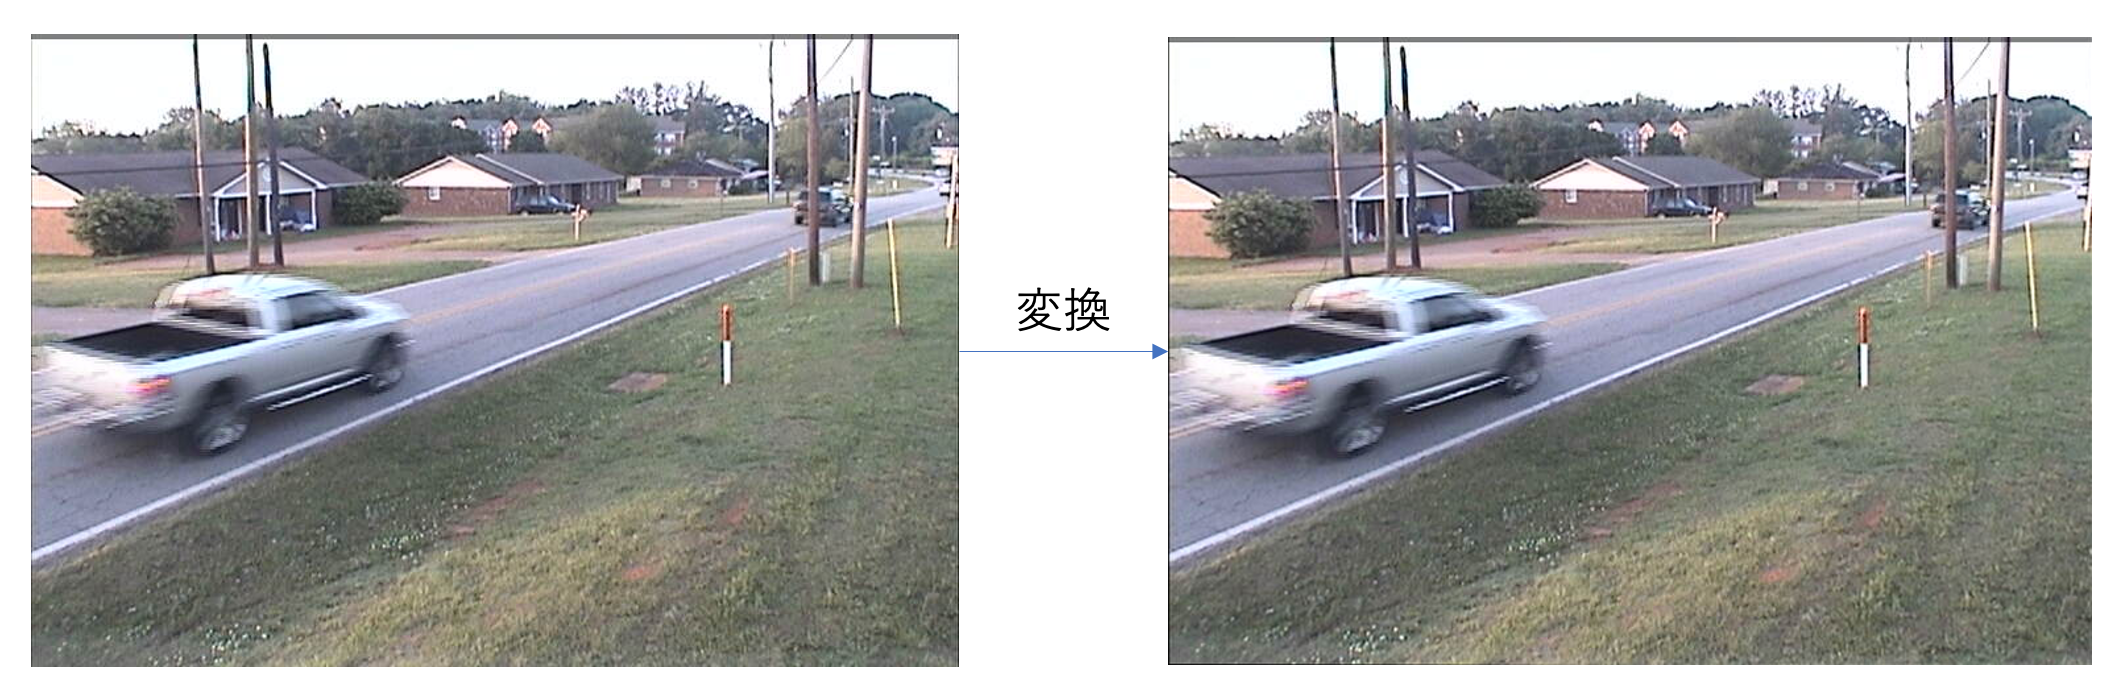
\includegraphics[width=13cm]{./problem_2}
    \caption{背景領域の特徴点のみから導出したホモグラフィ行列による変換}
  \end{center}
\end{figure}

\begin{figure}[h]
  \begin{center}
    \includegraphics[width=10cm]{./ukihashi_method.bmp}
    \caption{前景領域の粗さ}
  \end{center}
\end{figure}




\chapter{提案手法}

\section{既存手法の問題点に対する提案}

本節では,2.9節で解説した既存手法の問題点, 特に前景領域の特徴点の削除に対する対策を提案する. 本節の提案手法は,既存手法の改善であるため,補間フレームの前景領域の視覚的品質の改善が主となる. 本節で提案する手法の全体像を図[]に示す. 既存手法との主な変更点は, 前景領域の特徴点の利用である. 以下, 前景領域の高精細化までの流れを解説する.

\begin{figure}[h]
  \begin{center}
    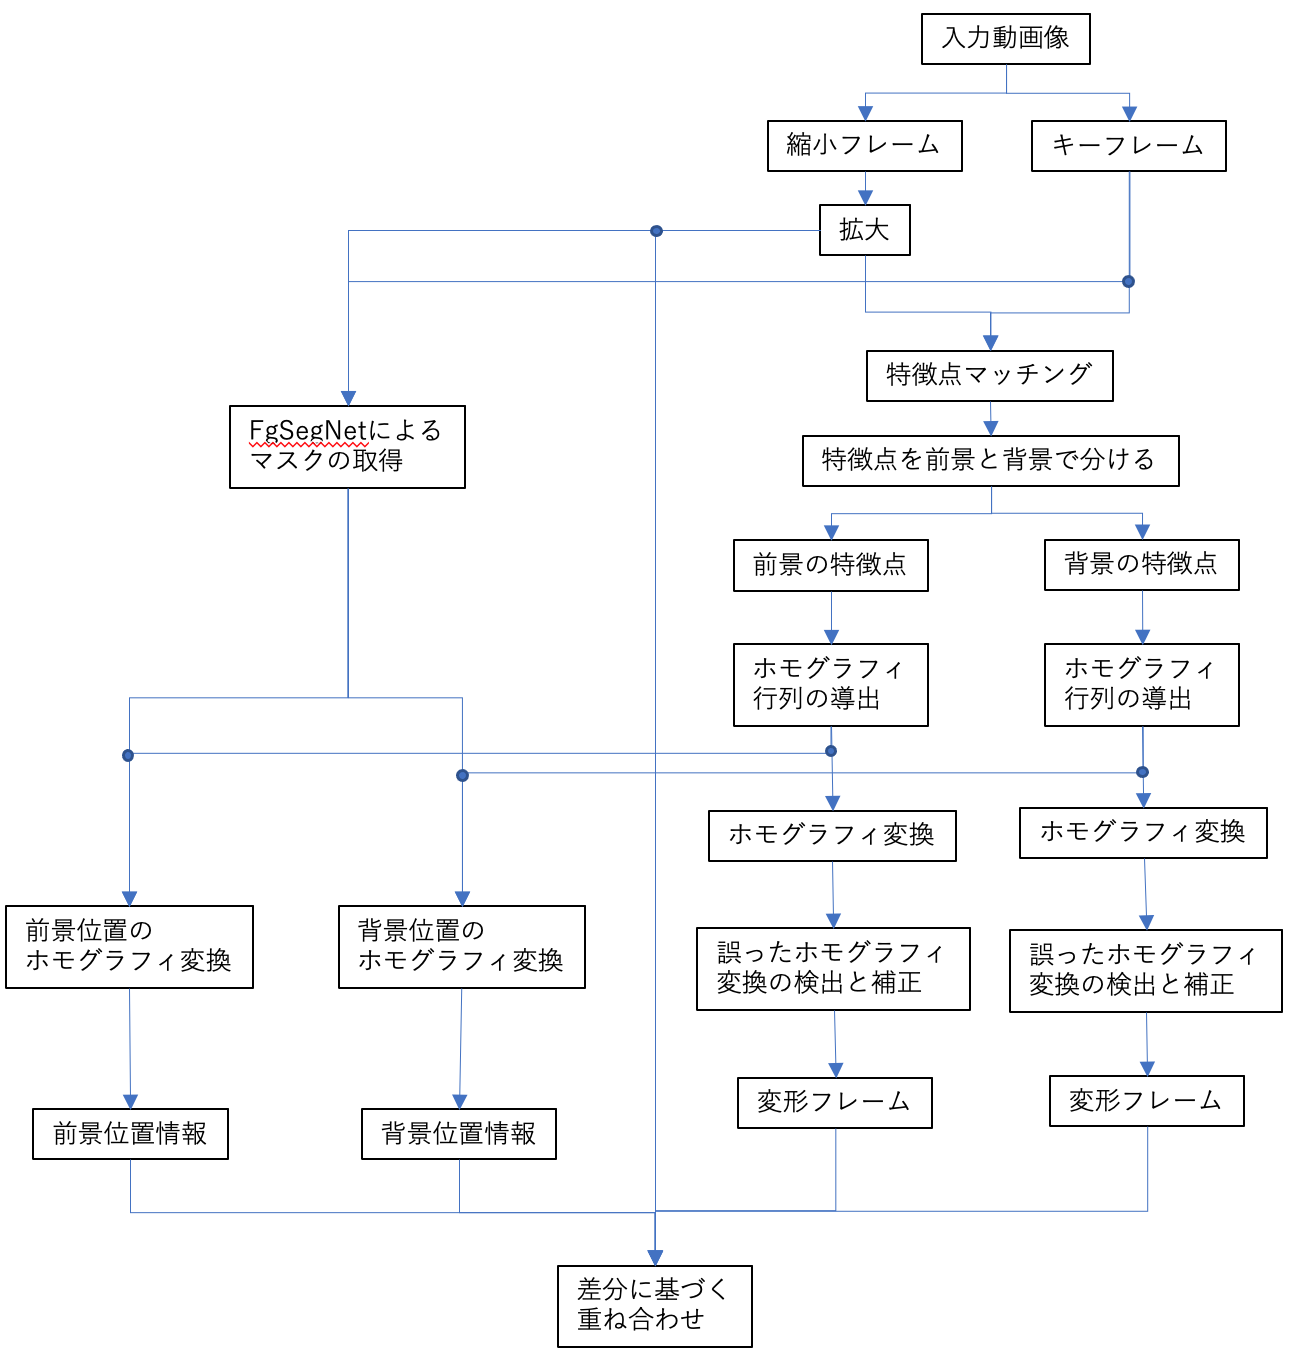
\includegraphics[width=10cm]{./zentaizou.png}
    \caption{提案手法の全体像}
  \end{center}
\end{figure}

\subsection{前景と背景の特徴点を分ける}
提案手法の問題点で説明したように, 既存手法では前景領域の特徴点を削除していた. そのため, ホモグラフィ変換をしたキーフレームは, 前景領域が移動せず, 最終的な補間フレームの前景領域は, 拡大フレームの前景領域の情報を用いていた. そこで提案手法では, 前景領域の特徴点を削除せずに, 前景領域と背景領域の特徴点を分けて, どちらの特徴点も利用する. 図[]のように, 対象の特徴点が前景と背景のどちらに属するかをFgSegNetから取得した前景領域の情報に基づいて判断する. ここで用いるFgSegNetから取得した前景領域の情報のことをマスクという. 特徴点の領域を判別した後, それに対応するベクトルに格納する. その後, それぞれのベクトルからホモグラフィ行列を求め, これを前景用のホモグラフィ行列と背景用のホモグラフィ行列とする.

\begin{figure}[h]
  \begin{center}
    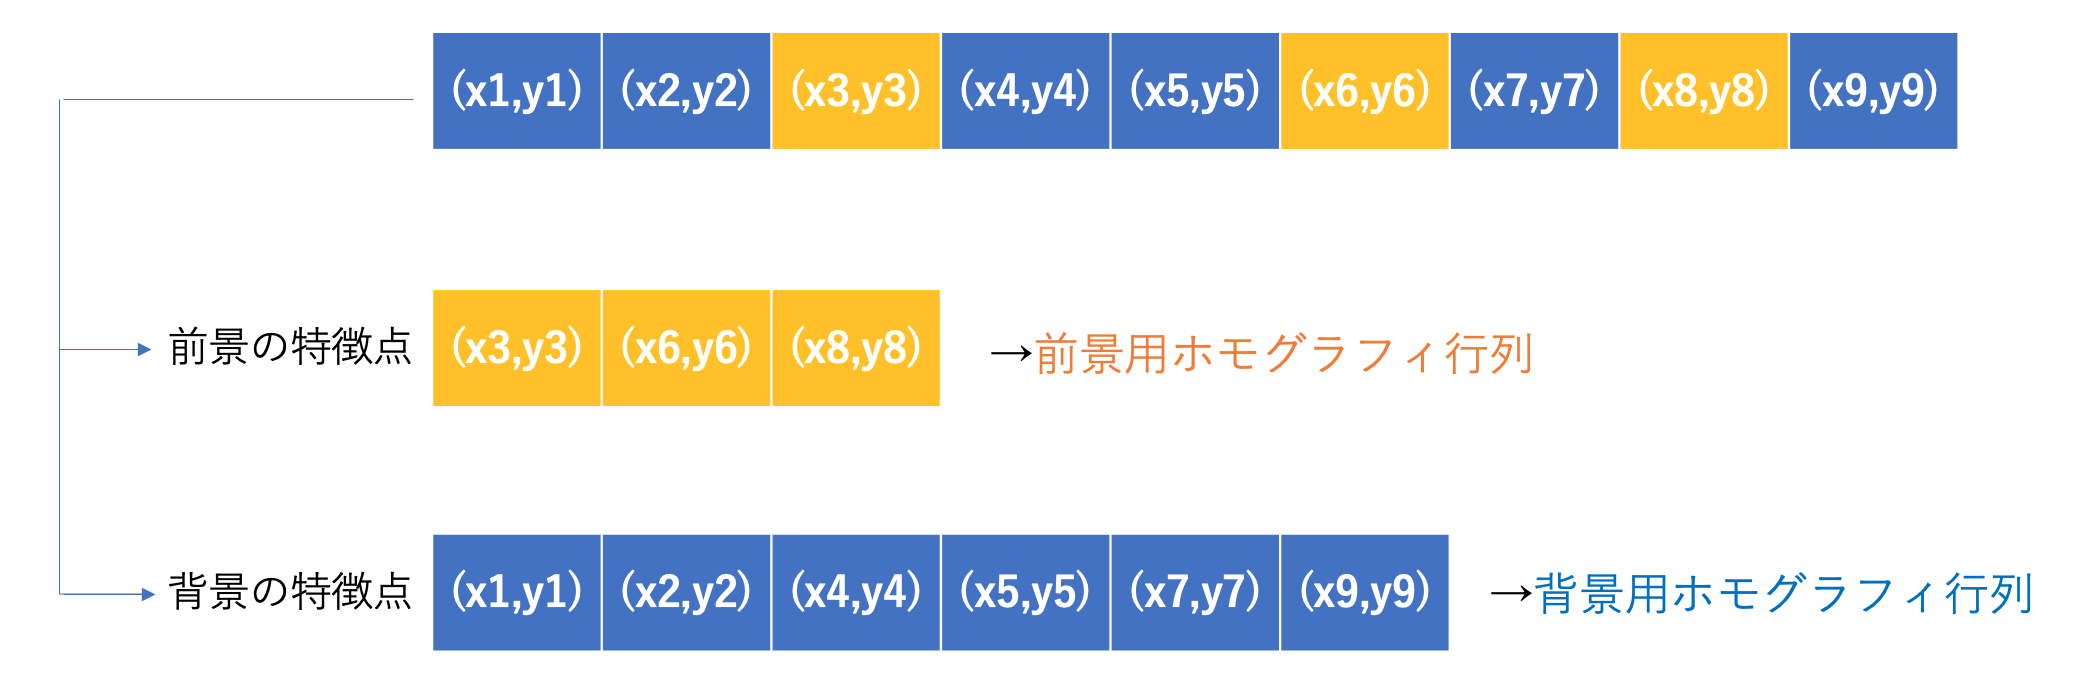
\includegraphics[width=10cm]{./teian_1.png}
    \caption{前景と背景で特徴点を分ける}
  \end{center}
\end{figure}

\subsection{前景と背景を別々にホモグラフィ変換}
前節で求めた2つのホモグラフィ行列を用い, それぞれでキーフレームのホモグラフィ変換を行う. 背景用ホモグラフィ行列で変換したキーフレームは, 既存手法と同様に, 背景の高精細化に用いる(図[]の右の図). 前景用ホモグラフィ行列で変換したキーフレームを図[]に示す. 図[]のように, 前景用ホモグラフィ行列で変換したキーフレームの前景領域は, 拡大フレームの前景領域とほぼ同じ位置に移動できていることがわかる. これを拡大フレームの前景領域の高精細化に用いる.

\begin{figure}[h]
  \begin{center}
    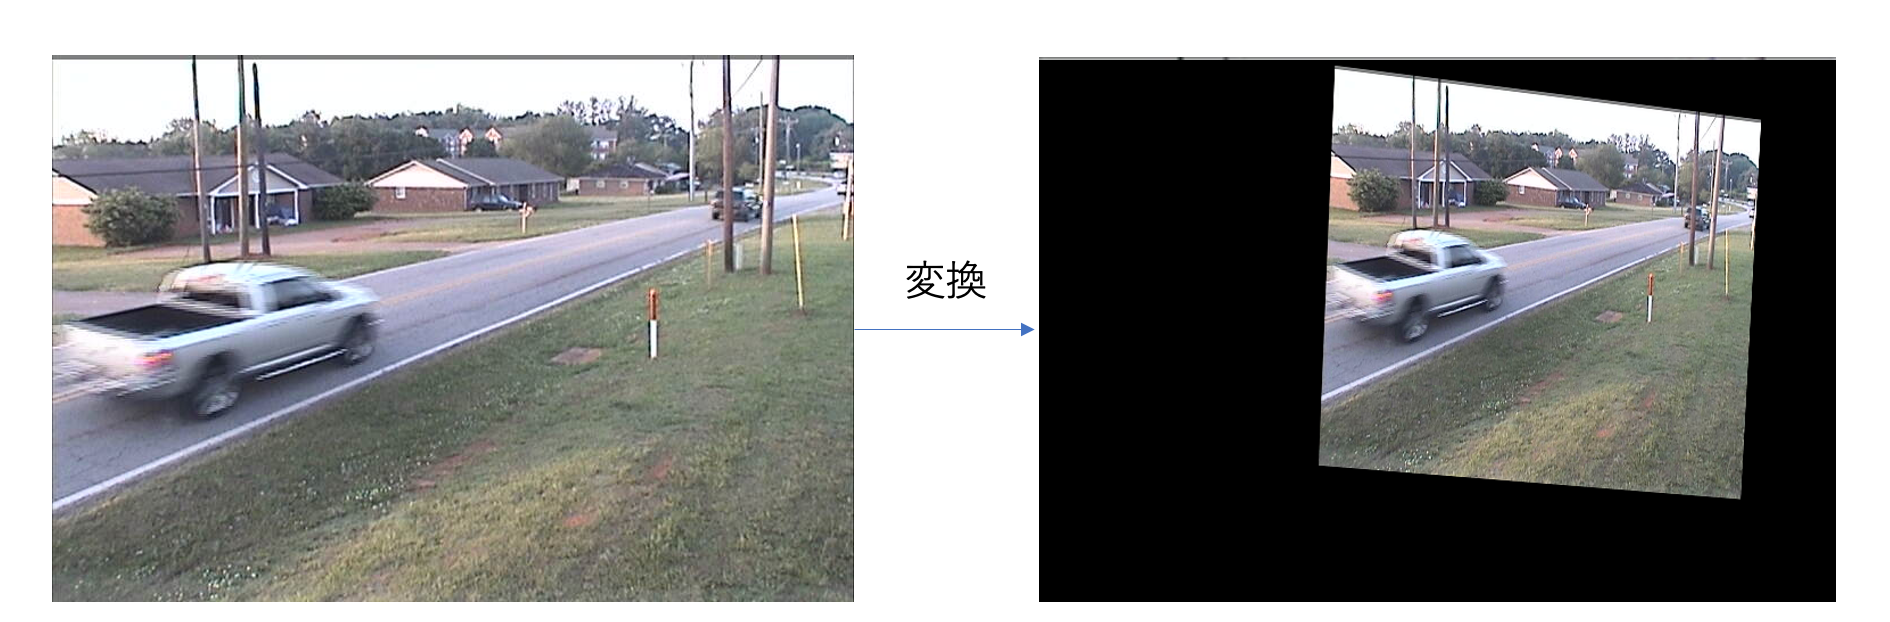
\includegraphics[width=13cm]{./teian_2.png}
    \caption{前景用ホモグラフィ行列で変換したキーフレーム}
  \end{center}
\end{figure}

\begin{figure}[h]
  \begin{center}
    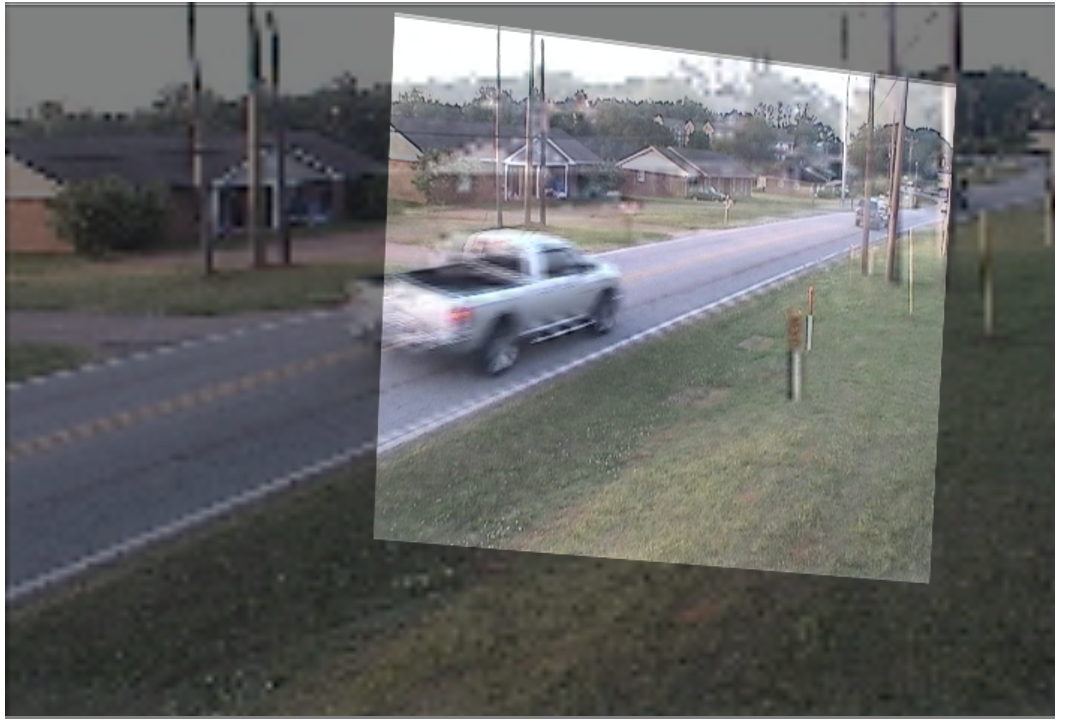
\includegraphics[width=10cm]{./teian_2_2.png}
    \caption{前景用ホモグラフィ行列で変換したキーフレームと拡大フレームの比較}
  \end{center}
\end{figure}


\subsection{前景と背景を別々に投影}
前節で求めた, 2枚の変形キーフレームを, 1枚ずつ拡大フレームに投影する.
まず初めに, 背景の投影を行う. 拡大フレームのマスクと背景用ホモグラフィ行列で変換したキーフレームを重ね, マスク上の白の領域と重なるキーフレームの領域を, 拡大フレームに投影する. この段階で, 背景のみが高精細化された補間フレーム(1*)が生成される. 
次に, 前景の投影を行う. ここでマスクの白黒を反転させ, 前景領域が白で表されるようにする. その後は背景の時と同様に, 拡大フレームのマスクと前景用ホモグラフィ行列で変換したキーフレームを重ね, マスク上の白の領域と重なるキーフレームの領域を, 前段階で出力した背景のみが高精細化された補間フレーム(1*)に投影する. こうすることで, 拡大フレームの前景と背景を共にキーフレームの情報に置き換えたことになる. 

\begin{figure}[h]
  \begin{center}
    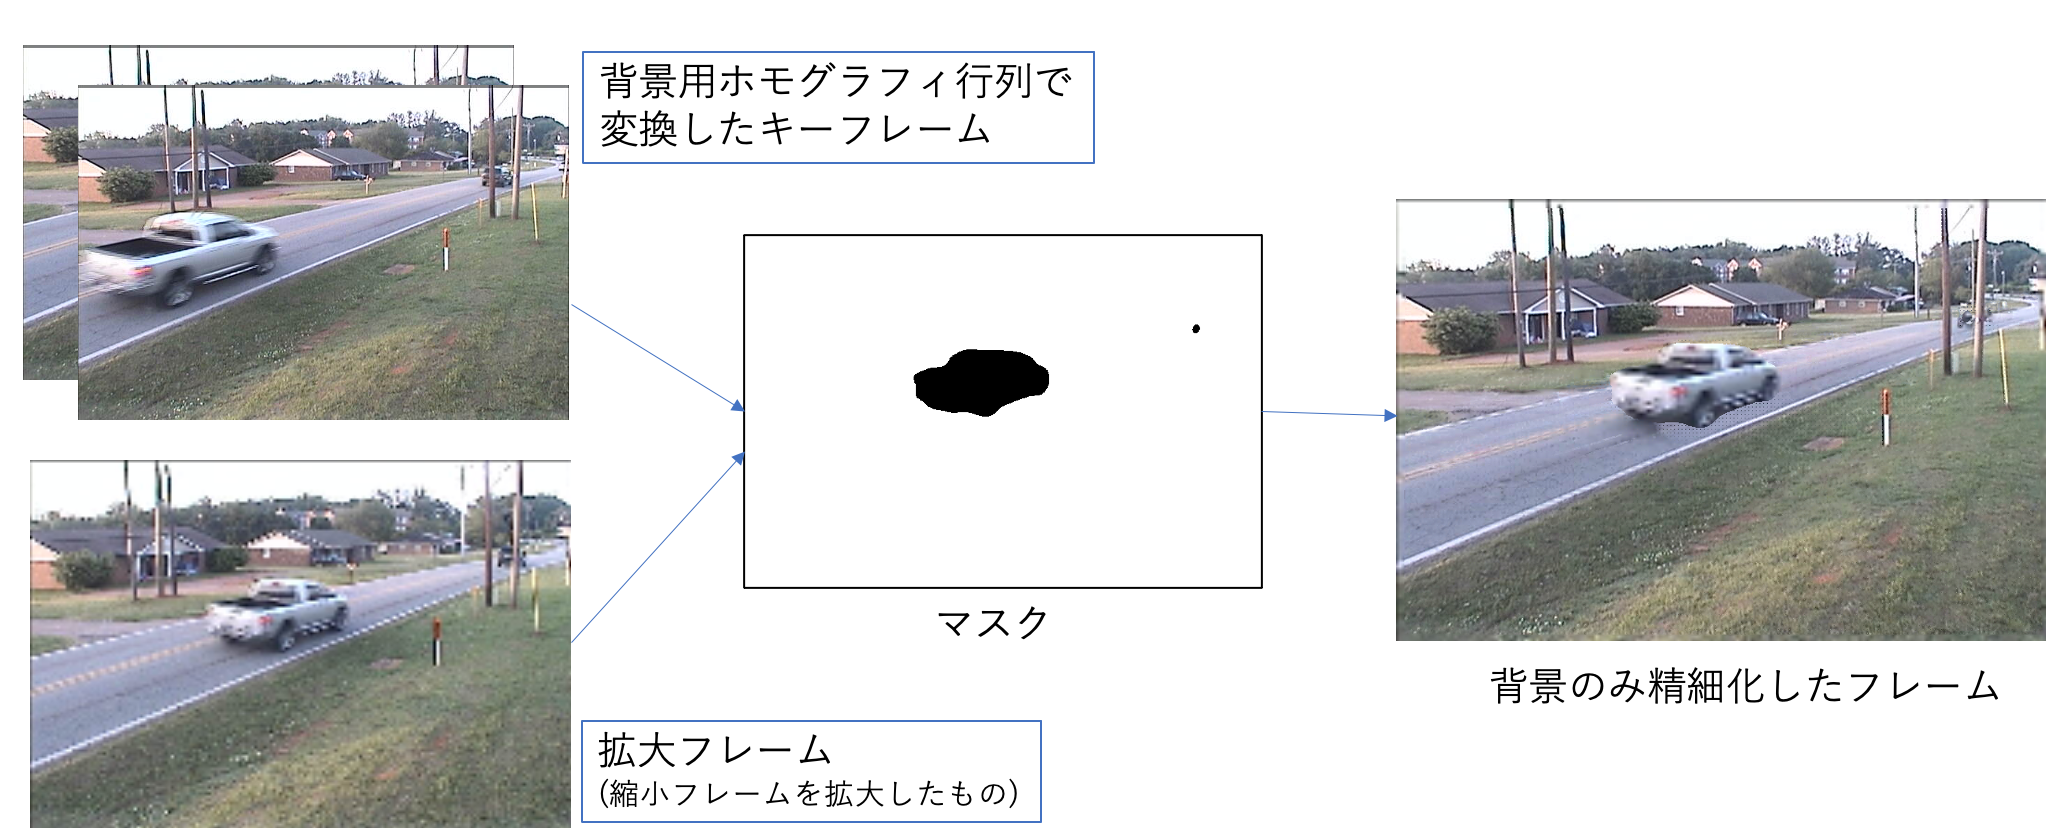
\includegraphics[width=10cm]{./teian_3_1.png}
    \caption{背景領域を投影}
  \end{center}
\end{figure}

\begin{figure}[h]
  \begin{center}
    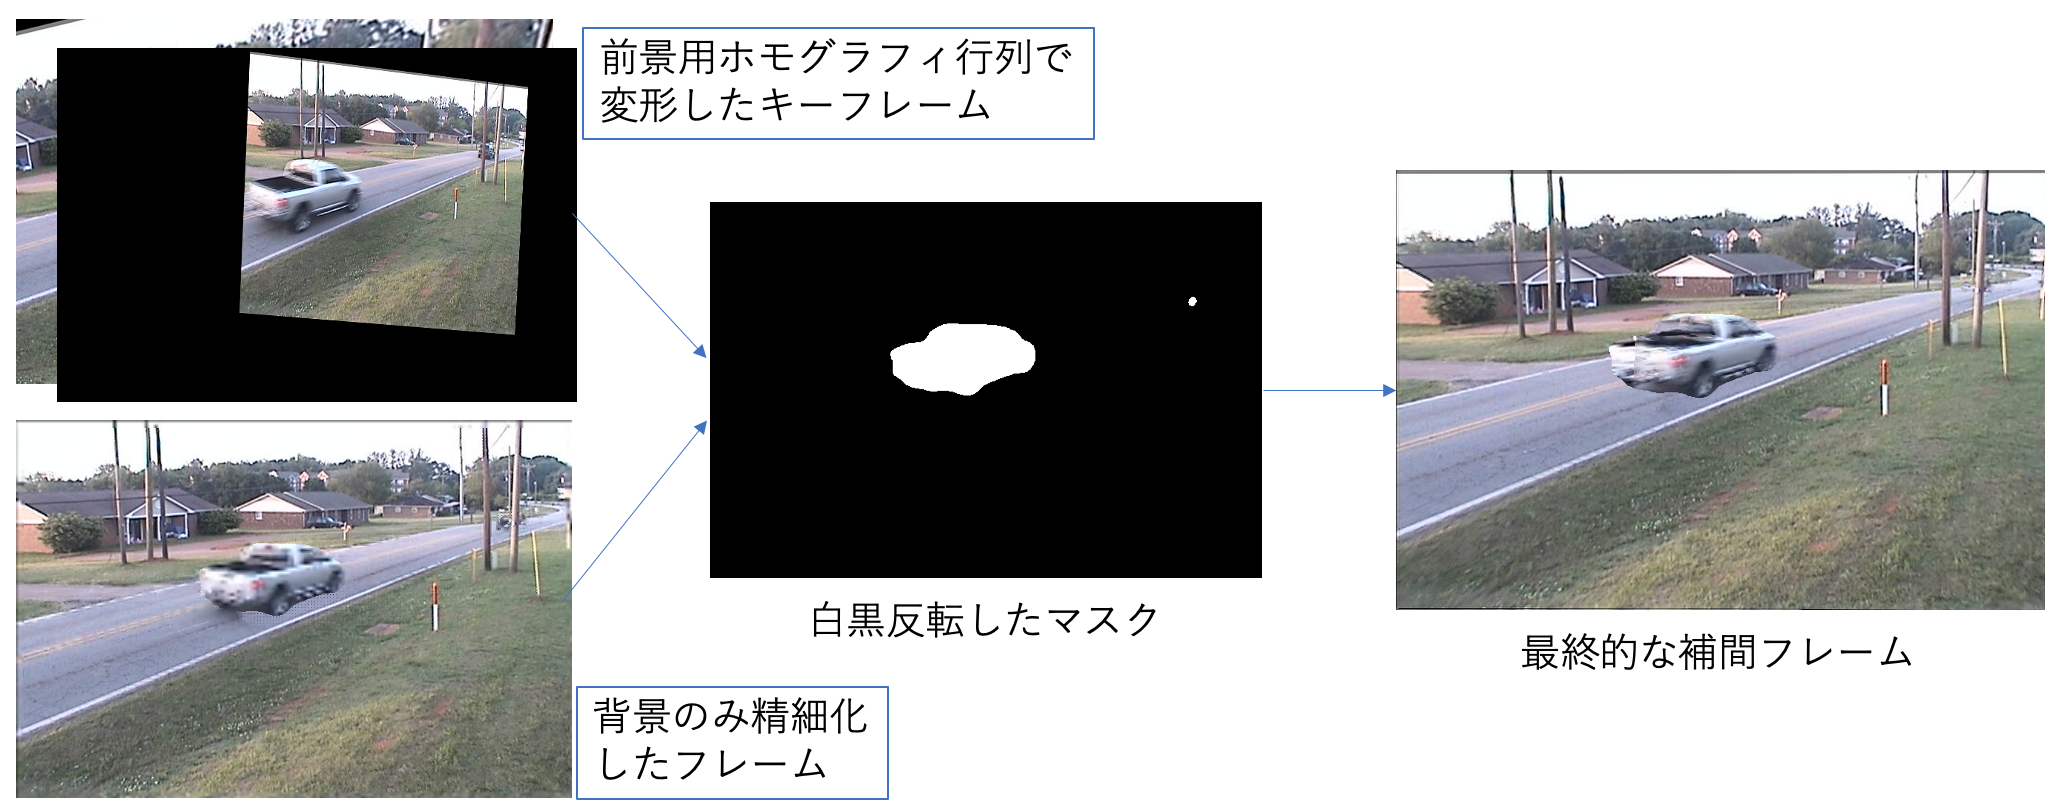
\includegraphics[width=10cm]{./teian_3_2.png}
    \caption{前景領域を投影}
  \end{center}
\end{figure}


\chapter{実験} 
本章では,3章で提案した手法の実験と考察を行う. まず,提案手法と既存手法の比較を行う. この章で性能評価に用いる動画像は CDnet2014[]の Continuous Pan である. キーフレームの間に 2枚の縮小フレームが存在するとし, 縮小フレームは縦横 1/4 に画素を間引いて作成する.

\section{提案手法の評価}
本節では, 3 節で提案した既存手法の問題点に対する提案 の評価を行う. 本節の手法は C++を用いて実装されている. この節では, 既存手法による補間フレームと提案手法による補間フレームを, PSNRとNIQEの観点からの評価と, 主観的な品質で比較をする. 補間手法としての比較は, データ量が少ないため, この実験結果をもとに考察を行うに留める. また, 提案手法を構成する各手法についての考察も行う. 

\subsection{PSNR,NIQEにおける評価}
表[]に各手法のPSNR, NIQEの値を示す. 提案手法は,既存手法よりPSNRの値は低いが, NIQEの値では上回っている. PSNRの低下の理由の一つとしては, 拡大フレームのピクセルの埋め込みを行っていないことが考えられる. 既存手法では, 補間フレームを生成した後, 最後の工程として, 拡大フレームのピクセル値を4ビット毎に埋め込んでいる. そのため, 画像の4分の1は差分が0となり, PSNRに影響を与えない. 提案手法では, その埋め込まれた拡大フレームのピクセルが主観的品質に影響を与えるという理由から, この工程は除いている. 
NIQEは, 値が小さい方が良いという指標であるため, NIQEの観点からは, 若干ではあるものの改善できていると言える. 

\begin{table}[h]
\begin{tabular}{ccc}
& 既存手法 & 提案手法\\
PSNR & 24.5069 & 23.5721\\
NIQE & 4.1464 & 3.8578
\end{tabular}
\end{table}


\subsection{主観による評価}
図[]に, 既存手法による補間フレームと提案手法による補間フレームを示す.  提案手法は既存手法に比べ, 明らかに前景領域が精細に補間できていることがわかる. これは, 前景を適切な位置にホモグラフィ変換したことによるものである. 以上より, 提案手法は, 前景領域の主観的品質において, 既存手法より高い性能を示していると考える. しかし, 比較的に改善されたとは言え, いくつかの課題は残されている. 以降の小節は, 提案手法を構成する各手法と, それに関連する課題を考察する. 

\begin{figure}[h]
  \begin{center}
    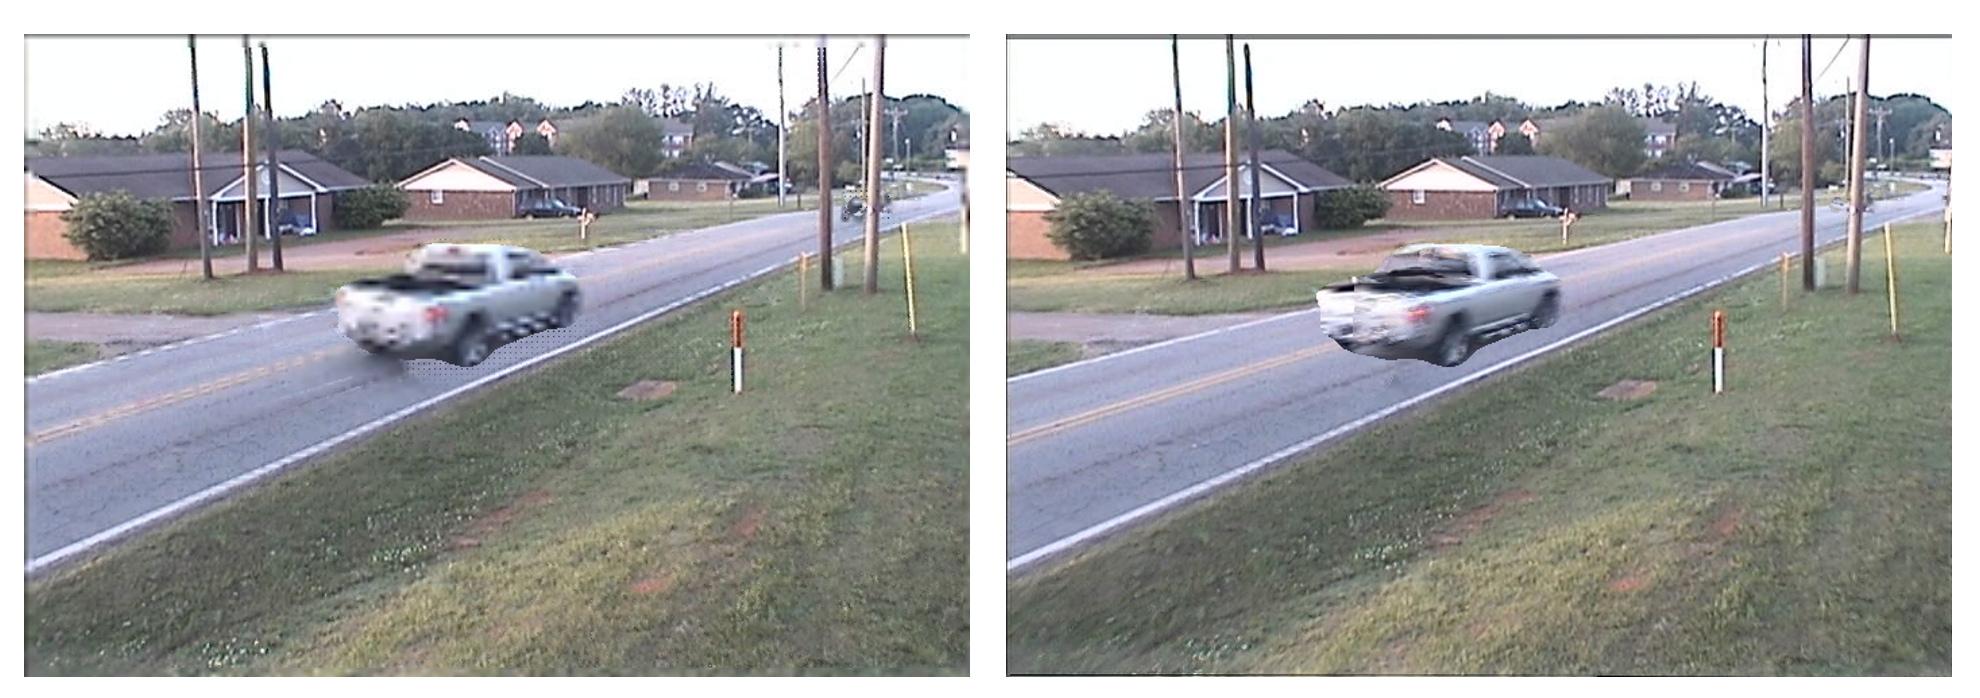
\includegraphics[width=10cm]{./kekka.png}
    \caption{既存手法(左), 提案手法(右)による補間フレーム}
  \end{center}
\end{figure}

\section{課題と考察}

\subsection{課題1. 前景領域の欠損}
図[]に示した補間フレームと別の時刻のものを図[]に示す. これより, 前景領域の一部が欠けていることがわかる. 理由の一つとしては, FgSegNetの前景領域の認識ミスが挙げられる. 図[]は, 拡大フレームの一部とその領域のFgSegNetの認識結果を示している. 前景が小さくなると, その領域を正確に認識できていないことがわかる. FgSegNetによって取得したマスクは, 投影の際に用いているため, キーフレームのホモグラフィ変換が正確にできていたとしても, マスクにおける前景領域の部分以外はフィルタリングされ, 結果的に前景領域の一部がかけた補間フレームが生成されることになる. 


\begin{figure}[h]
  \begin{center}
    \includegraphics[width=10cm]{./zenkei_kieru.bmp}
    \caption{一部が欠けた前景領域}
  \end{center}
\end{figure}

\begin{figure}[h]
  \begin{center}
    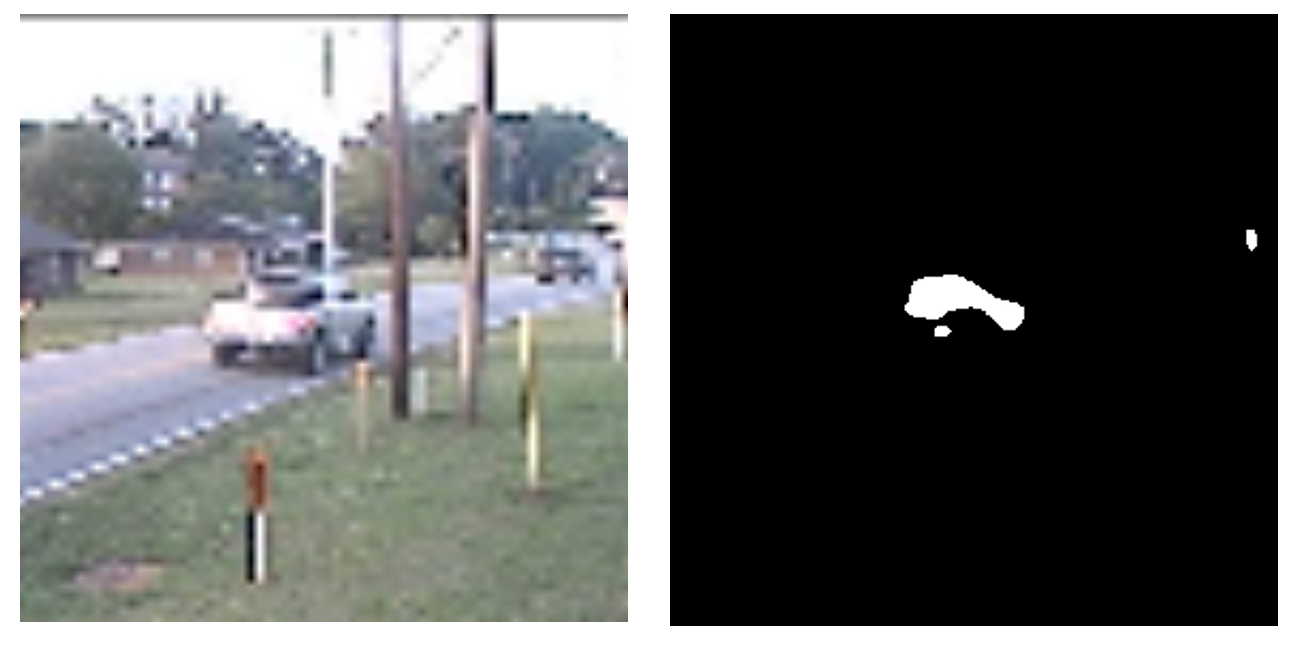
\includegraphics[width=10cm]{./fgsegnet_miss}
    \caption{前景領域の認識ミス}
  \end{center}
\end{figure}

\subsection{課題2. FgSegNetが前景と認識しない領域}
前節で示した問題が, FgSegNetが認識"できない"領域に関するものであるのに対し, FgSegNetが前景と認識"しない"領域も問題として挙げられる. 今回の例では, 車(前景)の影がそれに当たる.
図[]を見ると, 影の補間が全くできていないことがわかる. 図[]に, 拡大フレームの前景領域を, その時刻のマスクで切り抜いたものを示す. これより, FgSegNetが車の影の領域を前景とみなしていないことがわかる. 
(FgSegNetの仕組みについて簡単に触れる?)

\begin{figure}[h]
  \begin{center}
    \includegraphics[width=10cm]{./inada_method.bmp}
    \caption{影の補間ができていない}
  \end{center}
\end{figure}

\begin{figure}[h]
  \begin{center}
    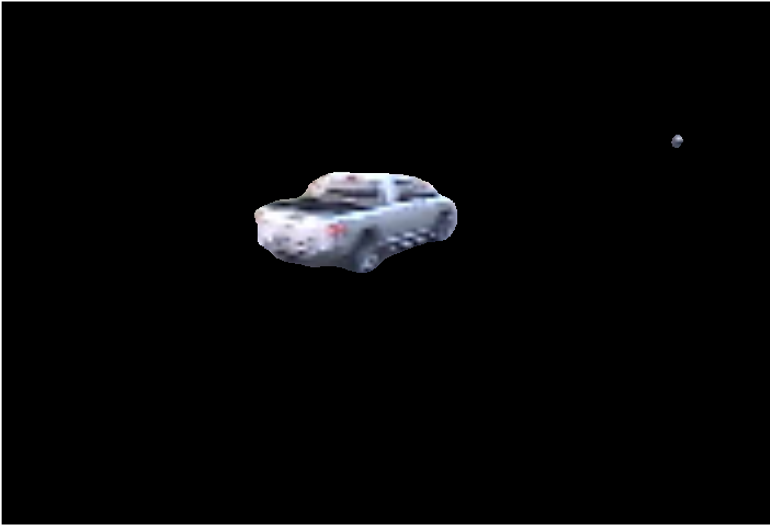
\includegraphics[width=10cm]{./fgsegnet_kage.png}
    \caption{マスクに影の領域が含まれない}
  \end{center}
\end{figure}


\section{考察}
前節までで示したように, FgSegNetの前景認識の結果は, 最終的に得られる補間フレームの視覚的品質に強く影響を与える. しかし, 補間フレームの前景に関する課題は, 最終的な投影の仕方に根本的な問題があると考える. 
既存手法と提案手法の投影の仕方における違いは, 前景領域を投影するかどうかという点のみであり, 変形キーフレーム.拡大フレーム.マスクを用いるという点では同じである. 現状としては, 変形キーフレームと拡大フレームの間にマスクを挟み, マスクをフィルターとして変形キーフレームの情報を拡大フレームに投影している. そのため, 変形キーフレームの前景領域が拡大フレームの前景領域と同じ位置にあったとしても, マスク上でその領域は背景だと認識されていれば, 変形キーフレームの情報はフィルタリングされ, 拡大フレームに投影されないことになる. 
本来であれば, キーフレームの情報に置き換えるというより, 図[]のように変形キーフレームと拡大フレーム,,,をバランスよく配合する重ね合わせをすべきと言える. このような重ね合わせの仕方に改良した上で, 各フレームの情報の利用率の最適化が今後の課題であると考える. 

\begin{figure}[h]
  \begin{center}
    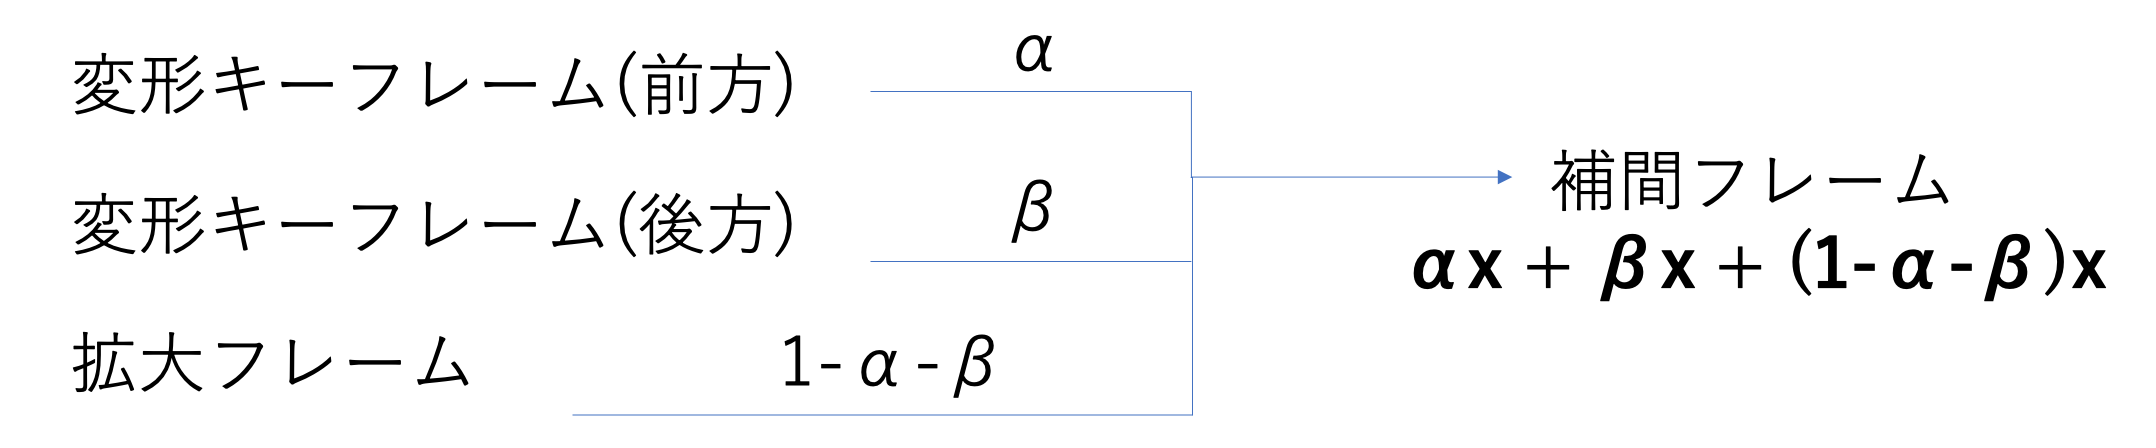
\includegraphics[width=10cm]{./honrai_kasaneawase.png}
    \caption{本来の重ね合わせの手法}
  \end{center}
\end{figure}


\chapter{終わりに}
本稿では,動画像のデータ量削減を目的とした 2 種類の解像度のフレームが混在する動画像を用いたフレーム補間手法に注目し,既存手法による補間フレームの前景領域の視覚的品質の向上を目的としていた. そこで, 既存手法の問題点に対していくつかの対策を提案した. 一つ目の問題点として, 評価手法をあげた. 既存手法の評価が客観的指標のみによる評価だったことに対して, NR-IQAモデルの一つであるNIQEを導入することで, 主観と客観という2つの指標による評価を行った. 二つ目の問題点として, 前景領域の品質をあげた. 既存手法では, 背景領域の高精細化を目的としていたため, 背景領域の特徴点のみを用いて, フレーム補間を行なっていた. これに対しては, 前景領域の特徴点と背景領域の特徴点を別々に利用することで,背景領域の品質は維持しつつ, より精細な前景領域の補間を試みた. しかし, 重ね合わせの仕方という問題が明らかになった. 
今後は, 重ね合わせの仕方を根本的に変更した上で, 各フレームの情報の最適な利用率を求めることで, 更なる品質の向上が期待できると考える. 



\chapter*{謝辞}
本研究にあたり,ご指導をして頂いた越智裕之教授,今川隆司助教に 心より感謝致します.また,日頃より研究についてご討論頂いた,集積 システム研究室の諸氏に心より感謝致します.最後に学業に専念できる よう私生活を支えて頂いた両親に深く感謝致します.

\bibliography{ref.bib}

\end{document}







